% ---------------------------------------------------------------------------
% IESB - Graduação em Ciência de Dados e Inteligência Artificial
% Template para desenvolvimento do Trabalho de Conclusão do Curso
% Este template teve como ponto de partida o template do curso de 
% Engenharia da Computação do IESB
% Adaptação Professores Sérgio Côrtes e Suélio Moura
% ---------------------------------------------------------------------------
%\documentclass[12pt,openright,twoside,a4paper,brazil]{abntex2}
\documentclass[
	12pt,				% tamanho da fonte			
	a4paper,			% tamanho do papel
                    	% opções do pacote babel
    openany,            % As três classes de documentos padrão mais comumente usadas em LaTeX incluem: artigo, relatório e livro.
    twoside,            % oneside: impressão só frente - twoside: impressão em frente e verso. Controle das marges do documento (O LATEX oferece a possibilidade de declarar o documento como unilateral ou bilateral, isto irá organizar vários elementos para que fiquem bem no formato escolhido. - twoside)
	english,			% idioma adicional para hifenização
%	french,				% idioma adicional para hifenização
	spanish,			% idioma adicional para hifenização
	brazil,				% idioma principal do documento (último na declaração)
	]{abntex2}          %

% {abntex2} O abnTeX2, evolução do abnTeX (Normas ABsurd para TeX *), é uma suíte para LaTeX que atende os requisitos das normas da ABNT (Associação Brasileira de Normas Técnicas) para elaboração de documentos técnicos e científicos brasileiros, como artigos científicos, relatórios, trabalhos acadêmicos como teses, dissertações, projetos de pesquisa e outros documentos do gênero.

% ---------------------------------------------------------------------------
% PACOTES para construção do documento
% ---------------------------------------------------------------------------

% ---------------------------------------------------------------------------
% Pacotes fundamentais 
% ---------------------------------------------------------------------------

\usepackage[utf8]{inputenc}		% Codificação do documento (conversão automática dos acentos)
\usepackage{indentfirst}		% Indenta o primeiro parágrafo de cada seção.
\usepackage{color}	
\usepackage{xcolor} % Controle das cores
\usepackage{graphicx}			% Inclusão de gráficos
\usepackage{microtype} 			% para melhorias de justificação
\usepackage[toc,page]{appendix}

% ---------------------------------------------------------------------------
\usepackage{pdfpages} % permite inserir páginas em pdf
% ---------------------------------------------------------------------------
\usepackage{setspace} % permite inserir notas em tabelas
\usepackage{threeparttable}
% ----------------------------------------------------------
\usepackage{verbatim}			% pacote para adicionar comentários em bloco
% ----------------------------------------------------------
% Pacotes adicionais, usados no anexo do modelo de folha de identificação e cronograma
% ----------------------------------------------------------
\usepackage{multicol}
\usepackage{multirow}
\usepackage{pgfgantt}     %pacote do gráfico de gantt
\usepackage{hyperref}     %pacote para adicionar links internos

% ----------------------------------------------------------
% Pacotes adicionais, usados apenas no âmbito do Modelo Canônico do abnteX2

% ----------------------------------------------------------
% Pacotes de citações
% ----------------------------------------------------------
\usepackage[brazilian,hyperpageref]{backref}	 % Paginas com as citações na bibl
%\usepackage[num]{abntex2cite}	% Citações padrão ABNT
\usepackage[alf]{abntex2cite}	% Citações padrão ABNT
\usepackage{listings}


%\usepackage{cite}
%\renewcommand\citeleft{(}
%\renewcommand\citeright{)}

% ----------------------------------------------------------
% CONFIGURAÇÕES DE PACOTES
% ----------------------------------------------------------

% Configurações do pacote backref
% Usado sem a opção hyperpageref de backref
\renewcommand{\backrefpagesname}{Citado na(s) página(s):~}
% Texto padrão antes do número das páginas
\renewcommand{\backref}{}
% Define os textos da citação
\renewcommand*{\backrefalt}[4]{
	\ifcase #1 %
		Nenhuma citação no texto.%
	\or
		Citado na página #2.%
	\else
		Citado #1 vezes nas páginas #2.%
	\fi}%
% ---

% ---
% Configurações de aparência do PDF final

% alterando o aspecto da cor azul
\definecolor{blue}{RGB}{41,5,195}

% informações do PDF
\makeatletter
\hypersetup{
     	%pagebackref=true,
		pdftitle={\@title}, 
		pdfauthor={\@author},
    	pdfsubject={\imprimirpreambulo},
	    pdfcreator={LaTeX with abnTeX2},
		pdfkeywords={abnt}{latex}{abntex}{abntex2}{gestão participativa}{gênero feminino}{IFTO}, 
		colorlinks=true,       		% false: boxed links; true: colored links
    	linkcolor=blue,          	% color of internal links
    	citecolor=blue,        		% color of links to bibliography
    	filecolor=magenta,      		% color of file links
		urlcolor=blue,
		bookmarksdepth=4
}
\makeatother
% --- 

% --- 
% Espaçamentos entre linhas e parágrafos 
% --- 

% O tamanho do parágrafo é dado por:
\setlength{\parindent}{1.3cm}

%espaçamento entre capítulos e o texto subsequente
\setlength{\afterchapskip}{1cm}

% Controle do espaçamento entre um parágrafo e outro:
\setlength{\parskip}{0.2cm}  % tente também \onelineskip

% ---
% compila o indice
% ---
\makeindex
% ---

% ----
% Início do documento
% ----
\begin{document}


% Seleciona o idioma do documento (conforme pacotes do babel)
%\selectlanguage{english}
\selectlanguage{brazil}

% Retira espaço extra obsoleto entre as frases.
\frenchspacing 

% ----------------------------------------------------------
% ELEMENTOS PRÉ-TEXTUAIS
% ----------------------------------------------------------
% \pretextual

% ----------------------------------------------------------------------------
% Capa do TCC
% ----------------------------------------------------------------------------

\thispagestyle{empty}
\begin{center}
 \includegraphics[width=0.30\textwidth]{Figuras/iesb_Logo}
 \vspace*{1 mm}
\end{center}
\begin{center}
\vspace{1 mm}
   \begin{minipage}[b]{0.9\linewidth}
     \begin{center}
       \vspace{1cm}
       {\textbf{\Large {CENTRO UNIVERSITÁRIO INSTITUTO DE EDUCAÇÃO SUPERIOR DE BRASÍLIA}}} 
       {\textbf{\Large Bacharelado em \\ Ciência de Dados e Inteligência Artificial}}\\
        \vspace{1cm}
       {\textbf{\Large \textit{Trabalho de Conclusão de Curso I - TCC-I}}}
     \end{center}
   \end{minipage}
\end{center}

\vspace{8 mm}

\begin{center}
   {\textbf{\Large  \textbf{Vinícius de Paula R Carvalho}}}\\[2 cm]
   {\textbf{\Large Uma abordagem híbrida de mineração de texto e aprendizado não supervisionado para análise de comentários do Instagram dos governadores brasileiros. }}\\[2cm]
   {\textbf{\Large Brasília \\  2025}}\\[5cm]
   \vfill
\end{center}

% ---------------------------------------------------------------------------- %
% Página de rosto (SÓ PARA A VERSÃO DEPOSITADA - ANTES DA DEFESA)
% Resolução CoPGr 5890 (20/12/2010)
%
% IMPORTANTE:
%   Coloque um '%' em todas as linhas
%   desta página antes de compilar a versão
%   final, corrigida, do trabalho
%
%
\newpage
\thispagestyle{empty}
    \begin{center}
        \vspace{1.5 cm}
        \textbf{\LARGE{Uma abordagem híbrida de mineração de texto e aprendizado não supervisionado para análise de comentários do Instagram dos governadores brasileiros.}}\\ [3cm]
        \vspace{1.5 cm}
    \end{center}

   
     \hspace{.42\textwidth}
     \begin{minipage}{.52\textwidth}
Trabalho de Conclusão de Curso (TCC) apresentado como pré-requisito para obtenção de Bacharelado em Ciência de Dados e Inteligência Artificial pelo Instituto de Educação Superior de Brasília - IESB. \\ 
\textbf{Orientador:} Professor Sérgio da Costa Côrtes
    \end{minipage}

\pagebreak

% ---------------------------------------------------------------------------- %
%
% IMPORTANTE:
%   Coloque um '%' em todas as linhas
%   desta página antes de compilar a versão
%   final, corrigida, do trabalho
%
%
\newpage

\clearpage
\begin{center} 
    \textbf{\LARGE Uma abordagem híbrida de mineração de texto e aprendizado não supervisionado para análise de associações de marca dos governadores brasileiros. }\\[0.5cm]

    \textbf{{\large Vinícius de Paula R Carvalho}}\\[1.5cm]
\end{center}

\hspace{0.85cm}Trabalho de Conclusão de Curso (TCC) apresentado como pré-requisito para obtenção de Bacharelado em Ciência de Dados e Inteligência Artificial
pelo Instituto de Educação Superior de Brasília - IESB 

\vspace{1cm}

\hspace{0.85cm} Brasília – Distrito Federal, em \rule{1.5cm}{0.005cm} de \rule{3cm}{0.005cm} de \rule{1.5cm}{0.005cm}

\vspace{3cm}

\hspace{0.85cm}Banca Examinadora constituída pelos Professores:

\vspace{1cm}
\begin{center}\rule{10cm}{0.005cm}\\
    {\textbf {Profª. Drª. Fulana de Tal - Orientadora\\
    Professor no IESB}}
    
    \vspace{1cm}
    \rule{10cm}{0.005cm}\\
    {\textbf {Prof. Dr. Fulano de Tal - Membro \\
    Professor no IESB}}
    
    \vspace{1cm}
    \rule{10cm}{0.005cm}\\
    {\textbf {Prof. Dr. Fulano de Tal - Membro Externo \\
    Professor na UnB}}
    
    \vspace{1cm}
    \rule{10cm}{0.005cm}\\
    {\textbf{Prof. Dr. Fulano de Tal - Membro Externo \\
    Professor na ENCE}}

\end{center}

% ----------------------------------------------------------
% Agradecimentos
% ----------------------------------------------------------

\begin{agradecimentos}
Agradeço a DEUS pelo dom da vida e pela oportunidade de ter a família que tenho. Aos meus pais que sempre me proporcionaram um ensino de excelência, dentro de suas possibilidades. Agradeço, também, a todos os Professores do IESB que com seus conhecimentos, competências e habilidades me ensinaram e me prepararam para ser um profissional de excelência e um ser humano melhor.
\end{agradecimentos}
% ---

% ---
% Epígrafe
% ---
\begin{epigrafe}
    \vspace*{\fill}
	\begin{flushright}
		\textit{``Dados são iguais dentes,    \\
		só se joga fora em últico caso. \\
        Mas, ao usá-los a ética deve \\
        vir em primeiro lugar.''\\
		(Sérgio Côrtes)}
	\end{flushright}
\end{epigrafe}

% ----------------------------------------------------------
% RESUMO
% ----------------------------------------------------------

% !TEX root = TCC - CD e IA.tex
% ---
% RESUMO
% ---
% resumo na língua vernácula (obrigatório)
\setlength{\absparsep}{18pt} % ajusta o espaçamento dos parágrafos do resumo
\begin{resumo}
Este trabalho propõe o desenvolvimento e a validação de uma metodologia híbrida de mineração de texto que serve de motor a uma ferramenta de apoio à decisão para assessorias políticas. A abordagem integra técnicas de Processamento de Linguagem Natural (PLN) --- análise de sentimentos, para identificar polaridades; modelagem de tópicos, para extrair os temas centrais das discussões --- e aprendizado não supervisionado (clusterização), para agrupar publicações e perfis por características semelhantes. Diferentemente de abordagens que se encerram na descrição da opinião pública, os resultados dessas técnicas são organizados em um funil de engajamento inspirado no \textit{marketing} de crescimento (\textit{growth}) e nos construtos de \textit{Consumers' Online Brand-Related Activities} (COBRAs), convertendo a análise em recomendações práticas: o que produzir, o que amplificar e o que abandonar. A metodologia distingue o discurso produzido pelas assessorias --- em legendas e transcrições --- da reação expressa pelo público nos comentários, e é validada no estudo de caso dos vinte e sete governadores brasileiros. Espera-se que a pesquisa contribua com um instrumento analítico replicável para o marketing político digital, superando as limitações de métricas superficiais de engajamento ao qualificá-las pelo sentimento e organizá-las de forma acionável.

\vspace{0.5cm}
\noindent
\textbf{Palavras-chaves}: Marketing Político Digital, Análise de Sentimentos, Modelagem de Tópicos, Engajamento (COBRAs), \textit{Growth}, Ciência de Dados.
\end{resumo}

% ----------------------------------------------------------
% ABSTRACT
% ----------------------------------------------------------
% !TEX root = TCC - CD e IA.tex
% abstract em língua estrangeira (inglês)
%\setlength{\absparsep}{18pt} % ajusta o espaçamento dos parágrafos do resumo
\begin{otherlanguage*}{english}
This work proposes the development and validation of a hybrid text-mining methodology that serves as the engine of a decision-support tool for political communication teams. The approach integrates Natural Language Processing (NLP) techniques --- sentiment analysis, to identify polarities; topic modeling, to extract the central themes of the discussions --- and unsupervised learning (clustering), to group posts and profiles by similar characteristics. Unlike approaches that stop at describing public opinion, the results of these techniques are organized into an engagement funnel inspired by growth marketing and by the Consumers' Online Brand-Related Activities (COBRAs) framework, converting the analysis into actionable recommendations: what to produce, what to amplify, and what to abandon. The methodology distinguishes the discourse produced by the communication teams --- in captions and transcripts --- from the reaction expressed by the audience in the comments, and it is validated through a case study of Brazil's twenty-seven state governors. This research is expected to contribute a replicable analytical instrument for digital political marketing, overcoming the limitations of superficial engagement metrics by qualifying them through sentiment and organizing them in an actionable way.

\vspace{0.5cm}
\noindent
\textbf{Keywords}: Digital Political Marketing, Sentiment Analysis, Topic Modeling, Engagement (COBRAs), Growth, Data Science.
\end{otherlanguage*}

% ----------------------------------------------------------

\clearpage

% ----------------------------------------------------------
% inserir lista de ilustrações
% ----------------------------------------------------------
\pdfbookmark[0]{\listfigurename}{lof}
\listoffigures*
\cleardoublepage

% ----------------------------------------------------------
% inserir lista de tabelas
% ----------------------------------------------------------

\pdfbookmark[0]{\listtablename}{lot}
\listoftables*
\cleardoublepage

% ----------------------------------------------------------
% inserir lista de abreviaturas e siglas
% ----------------------------------------------------------
% ----------------------------------------------------------
% inserir lista de abreviaturas e siglas
% ----------------------------------------------------------
\begin{siglas}
    \item[API] Interface de Programação de Aplicativos (\textit{Application Programming Interface})
    \item[APP] Aplicativo (\textit{Application})
    \item[IBGE] Instituto Brasileiro de Geografia e Estatística
    \item[CD] Ciência de Dados (\textit{Data Science})
    \item[IA] Inteligência Artificial (\textit{Artificial Intelligence})
    \item[IoT] Internet das Coisas (\textit{IoT - Internet of things})
    \item[IP] \textit{Internet Protocol}
    \item[LBS] \textit{Location Based System}
   
\end{siglas}

% ----------------------------------------------------------
% inserir o sumario
% ----------------------------------------------------------
\pdfbookmark[0]{\contentsname}{toc}
\tableofcontents*
\cleardoublepage

% ----------------------------------------------------------
% ELEMENTOS TEXTUAIS
% ----------------------------------------------------------
\textual

% ----------------------------------------------------------
% Capítulos do Trabalho
% ----------------------------------------------------------

% !TEX root = ../TCC - CD e IA.tex
\chapter{INTRODUÇÃO}\label{INTRODUÇÃO}

Em um cenário no qual as mídias sociais se consolidaram como plataformas centrais para a comunicação e a formação da opinião pública, o volume massivo de dados gerados pelas interações de usuários \textemdash{} como os comentários no Instagram \textemdash{} emerge como uma fonte inestimável para a análise do engajamento político. Contudo, a natureza não estruturada e a escala desses dados tornam as abordagens analíticas manuais ou isoladas impraticáveis e superficiais \cite{JURAFSKY2025}. A lacuna não está apenas em compreender a polaridade do sentimento, os tópicos subjacentes ou a segmentação do público, mas em converter essa compreensão em decisão prática de comunicação: saber o que produzir, o que amplificar e o que abandonar. Diante disso, esta pesquisa propõe uma abordagem metodológica híbrida \textemdash{} combinando técnicas de Processamento de Linguagem Natural (PLN), como a análise de sentimentos e a modelagem de tópicos, e métodos não supervisionados, como a clusterização \textemdash{} e a articula a um funil de engajamento inspirado no \emph{marketing} de crescimento \cite{FEROZ2024} e nos construtos de \emph{Consumers' Online Brand-Related Activities} (COBRRas) \cite{MUNTINGA2011}. A análise não se limita aos comentários: abrange também as legendas e as transcrições da fala dos vídeos, contrastando o discurso produzido pelas assessorias com a reação expressa pelo público. Aplicada ao estudo de caso dos governadores brasileiros, a proposta visa demonstrar que a integração sinérgica dessas ferramentas supera as limitações das análises tradicionais, entregando não apenas uma leitura mais profunda das dinâmicas de opinião, mas um instrumento replicável de apoio à decisão para o marketing político e a comunicação organizacional.

\section{Contextualização e Definição do Problema}

A ascensão das plataformas de mídias sociais transformou o cenário da comunicação política e da formação da opinião pública. O Instagram, em particular, com sua natureza visual e sua capacidade de gerar engajamento massivo por meio de comentários, curtidas e visualizações, tornou-se um palco onde a percepção da figura política é moldada e expressa. Nesse contexto, a grande quantidade de dados gerados diariamente \textemdash{} textuais e quantitativos \textemdash{} representa um desafio significativo: a extração de inteligência e de \emph{insights} acionáveis de um volume tão grande e heterogêneo de informação.

O problema de pesquisa central reside na incapacidade das metodologias analíticas tradicionais, que frequentemente aplicam técnicas de forma isolada \textemdash{} apenas a análise de sentimento ou apenas a modelagem de tópicos \textemdash{}, de capturar a complexidade e a multidimensionalidade da percepção pública. Tais abordagens fragmentadas falham em identificar as nuances do discurso, os temas específicos que impulsionam um determinado sentimento e, crucialmente, em agrupar publicações e perfis com base em semelhanças que revelem padrões de desempenho e de comportamento comunicacional. Falham, ainda, em confrontar sistematicamente aquilo que a assessoria comunica \textemdash{} nas legendas e nas transcrições de seus vídeos \textemdash{} com aquilo a que o público de fato reage, nos comentários.

Some-se a isso um segundo problema, de ordem prática: mesmo quando esses sinais são medidos, raramente são traduzidos em orientação de decisão. Métricas de superfície, como o volume de curtidas ou de comentários, são frequentemente tomadas como sinônimo de aprovação, ignorando que alto engajamento pode decorrer tanto de aclamação quanto de controvérsia. Assim, a ausência de uma metodologia integrada \textemdash{} que combine sentimentos, tópicos e clusterização em múltiplos níveis de agregação e que organize seus resultados em um funil acionável \textemdash{} deixa um vácuo duplo: no entendimento aprofundado do comportamento do eleitorado e na capacidade de estrategistas de comunicação de tomar decisões informadas em um ambiente digital dinâmico e volátil.

Diante desse vácuo duplo, este trabalho estrutura-se em torno da seguinte pergunta de pesquisa:

\begin{quote}
\emph{Como a integração de análise de sentimentos, modelagem de tópicos e clusterização, aplicada às múltiplas fontes textuais e métricas das publicações de perfis políticos no Instagram, pode ser organizada em um funil de engajamento capaz de orientar as decisões de crescimento (\emph{growth}) de uma assessoria \textemdash{} isto é, o que produzir, o que amplificar e o que abandonar?}
\end{quote}

Dessa questão central desdobram-se três perguntas específicas que guiam o desenvolvimento do estudo. Primeiro, em que medida a abordagem híbrida, ao integrar as três técnicas, revela padrões de percepção pública que as análises isoladas não capturam? Segundo, como o confronto entre o discurso das assessorias \textemdash{} veiculado nas legendas e transcrições \textemdash{} e a reação do público \textemdash{} expressa nos comentários e nas métricas \textemdash{} pode qualificar o diagnóstico de desempenho de um perfil? Terceiro, de que forma os resultados dessa análise podem ser mapeados em estágios de um funil de engajamento, de modo a produzir recomendações práticas e replicáveis para a comunicação política digital?

\section{Relevância e Motivação}

A relevância e a motivação deste estudo residem na lacuna crítica entre a proliferação de dados de mídias sociais e a carência de metodologias analíticas robustas, integradas e \emph{orientadas à decisão} para extrair \emph{insights} significativos. Academicamente, a pesquisa contribui para os campos da Ciência de Dados, da Comunicação Social e do Marketing Político ao propor e validar um \emph{framework} analítico híbrido que transcende as limitações das abordagens tradicionais e isoladas de PLN. Ao demonstrar como a combinação sinérgica de análise de sentimentos, modelagem de tópicos e clusterização pode revelar padrões complexos de opinião \textemdash{} e ao organizar esses padrões segundo os construtos de engajamento dos COBRAs \cite{MUNTINGA2011} e a lógica do funil de \emph{marketing} de crescimento \cite{FEROZ2024} \textemdash{}, o estudo estabelece uma nova fronteira metodológica para a pesquisa aplicada em mídias sociais \cite{PANG2008}.

A motivação principal é suprir uma necessidade prática e urgente: oferecer a estrategistas de marketing político e a comunicadores organizacionais ferramentas que permitam ir além de métricas superficiais, como curtidas e compartilhamentos, proporcionando uma compreensão profunda e, sobretudo, \emph{acionável} da percepção pública e dos temas que efetivamente ressoam com o eleitorado. Em um ambiente político polarizado, no qual a comunicação digital é decisiva, torna-se um diferencial estratégico a capacidade de identificar não apenas o que o público sente, mas por que se sente assim, como os diferentes segmentos de opinião se organizam e \textemdash{} criticamente \textemdash{} em que medida o discurso produzido pela assessoria dialoga com aquilo a que o público de fato reage. O presente trabalho, ao focar nos governadores brasileiros, oferece um estudo de caso oportuno e de grande impacto, ilustrando a aplicação prática da metodologia para informar a tomada de decisão e aprimorar estratégias de engajamento.

\section{Visão Geral do Método}

A metodologia foi concebida como um pipeline de engenharia de dados e mineração de texto, estruturado para processar, de forma integrada, tanto as fontes textuais quanto as métricas quantitativas das publicações. O processo teve início com a coleta, via API da APIFY, de um corpus abrangendo três fontes textuais distintas \textemdash{} os comentários dos usuários, as legendas (\emph{captions}) das publicações e as transcrições da fala dos vídeos \textemdash{} além das métricas de engajamento associadas a cada perfil, publicação do \emph{feed} e \emph{Reel}. A etapa de pré-processamento incluiu a limpeza e a normalização dos textos, com a remoção de \emph{stopwords} da língua portuguesa por meio do recurso correspondente da biblioteca \texttt{nltk}.

Para a análise de sentimentos, empregou-se o \emph{pipeline} de \emph{sentiment-analysis} da biblioteca \texttt{transformers}, com o modelo multilíngue \code{cardiffnlp/twitter-xlm-roberta-base-sentiment}, que classifica cada texto com um rótulo de polaridade (\emph{Positive}, \emph{Negative} ou \emph{Neutral}) e uma pontuação de confiança. A análise foi aplicada de forma diferenciada: aos comentários dos usuários \textemdash{} distinguindo publicações do \emph{feed} e \emph{Reels} \textemdash{} para aferir a reação do público, e às legendas e transcrições para caracterizar o sentimento do discurso produzido pelas assessorias.

A modelagem de tópicos foi realizada com a biblioteca BERTopic, selecionada por sua capacidade de gerar tópicos coerentes e interpretáveis. Para otimizar a representação textual, os \emph{embeddings} de sentenças foram gerados pelo modelo \code{rufimelo/bert-large-portuguese-cased-sts}, pré-treinado em português., pré-treinado em português. A representação dos documentos foi aprimorada com a inclusão de emojis como \emph{tokens}, por meio de sua conversão em texto (\emph{demojize}) e da configuração de um \texttt{CountVectorizer} com expressão regular customizada. Uma inovação da metodologia foi a utilização de um \emph{Large Language Model} (LLM), o Gemini API, para refinar os rótulos dos tópicos: por meio de uma classe \texttt{GeminiDocsRefiner}, uma amostra de comentários de cada tópico foi fornecida ao modelo, que gerou descrições detalhadas, elevando a interpretabilidade dos resultados. A modelagem foi conduzida separadamente sobre os comentários e sobre o discurso oficial (legendas e transcrições), permitindo contrastar os temas que emergem da audiência com aqueles pautados pelas assessorias.

A clusterização foi aplicada em múltiplos níveis de agregação. No nível das publicações, as métricas de engajamento \textemdash{} previamente reduzidas por Análise de Componentes Principais (ACP) \textemdash{} alimentaram um procedimento de clusterização automática, conduzido tanto para os \emph{Reels} quanto para os posts do \emph{feed}, agrupando publicações por semelhança de desempenho. No nível dos perfis, o mesmo princípio foi aplicado às métricas agregadas dos governadores, agrupando-os por padrões de comportamento comunicacional. Por fim, os resultados das análises de sentimento, de tópicos e de clusterização foram integrados e mapeados em um funil de engajamento, articulando os níveis de COBRAs \cite{MUNTINGA2011} aos estágios do funil de crescimento \cite{FEROZ2024}, de modo a converter as evidências analíticas em recomendações práticas.

\section{Contribuições do Trabalho}

As principais contribuições deste trabalho desdobram-se em duas frentes: metodológica e prática. No âmbito metodológico, o estudo inova ao propor, desenvolver e validar uma abordagem analítica híbrida de Processamento de Linguagem Natural (PLN). Diferentemente de pesquisas que aplicam técnicas de forma isolada, esta integra análise de sentimentos, modelagem de tópicos e clusterização em um único pipeline coerente, aplicado a múltiplas fontes textuais \textemdash{} comentários, legendas e transcrições \textemdash{} e a diferentes níveis de agregação \textemdash{} publicações e perfis \textemdash{}, demonstrando que a sinergia dessas ferramentas oferece uma compreensão mais profunda e multifacetada do discurso nas redes sociais. A implementação vale-se de modelos e bibliotecas de ponta, como o \code{cardiffnlp/twitter-xlm-roberta-base-sentiment} para a análise de sentimento e o BERTopic para a modelagem de tópicos. Uma contribuição científica particularmente relevante é a incorporação de um \emph{Large Language Model} (LLM), o Gemini API, para refinar e gerar descrições interpretáveis dos tópicos identificados, elevando a qualidade e a utilidade dos resultados.

No campo prático, a contribuição central é a articulação dessa metodologia a um \emph{framework} acionável de crescimento (\emph{growth}). Ao mapear os resultados analíticos em um funil de engajamento \textemdash{} que integra os níveis de COBRAs \cite{MUNTINGA2011} aos estágios do funil de \emph{marketing} de crescimento \cite{FEROZ2024} \textemdash{}, o trabalho converte descrições da percepção pública em recomendações concretas de comunicação, orientando decisões sobre o que produzir, amplificar e abandonar. O confronto sistemático entre o discurso das assessorias (legendas e transcrições) e a reação do público (comentários e métricas) constitui, nesse sentido, um instrumento de diagnóstico original. Ao aplicar a proposta ao estudo de caso dos governadores brasileiros, a pesquisa fornece um exemplo concreto e replicável de como organizações podem extrair inteligência estratégica de grandes volumes de dados não estruturados do Instagram para aprimorar suas estratégias de engajamento.

\section{Estrutura e Organização do Trabalho}

Este trabalho está organizado em sete capítulos, seguindo uma progressão que parte da fundamentação conceitual, avança pela construção e aplicação da metodologia e culmina na tradução dos resultados em recomendações práticas.

O \textbf{Capítulo 1 \textemdash{} Introdução} contextualiza o problema, enuncia a pergunta de pesquisa e apresenta a relevância, a visão geral do método e as contribuições do estudo. O \textbf{Capítulo 2 \textemdash{} Objetivos} formaliza o objetivo geral e os objetivos específicos que orientam a pesquisa. O \textbf{Capítulo 3 \textemdash{} Referencial Teórico} reúne os fundamentos que sustentam o trabalho, abrangendo o marketing político digital e o \emph{marketing} de crescimento, a teoria de engajamento dos \emph{Consumers' Online Brand-Related Activities} (COBRAs), os precedentes de análise de audiência política em escala e os fundamentos de PLN \textemdash{} análise de sentimentos, modelagem de tópicos e clusterização.

O \textbf{Capítulo 4 \textemdash{} Fontes de Dados} descreve o corpus, sua origem e o processo de coleta das fontes textuais e das métricas de engajamento. O \textbf{Capítulo 5 \textemdash{} Modelagem} detalha o pipeline analítico e apresenta os resultados da análise exploratória, da redução de dimensionalidade, da clusterização, da análise de sentimentos e da modelagem de tópicos. O \textbf{Capítulo 6 \textemdash{} Resultados} consolida a aplicação do \emph{framework} de engajamento, articula os achados ao funil de crescimento e deriva, a partir do estudo de caso dos governadores, recomendações práticas por perfil e por tipo de publicação. Por fim, o \textbf{Capítulo 7 \textemdash{} Conclusões} sintetiza as contribuições, discute as limitações do estudo e aponta direções para trabalhos futuros.

\section{Cronograma e planejamento do trabalho}

A execução deste trabalho foi organizada em fases sequenciais, de modo a garantir a profundidade metodológica exigida por uma abordagem híbrida de mineração de dados. A primeira fase foi dedicada ao planejamento e à estruturação do trabalho, com a definição do problema de pesquisa e a elaboração do referencial teórico que forneceu a base conceitual para a análise.

Em seguida, procedeu-se à coleta e ao pré-processamento dos dados, etapa que envolveu a aquisição, via API, das fontes textuais e das métricas de engajamento dos perfis dos governadores, bem como o tratamento dos dados brutos \textemdash{} limpeza e normalização \textemdash{} para prepará-los para a análise.

O núcleo analítico do projeto correspondeu à fase de análise e modelagem, na qual as técnicas de Processamento de Linguagem Natural (PLN) foram aplicadas de forma integrada: a análise de sentimentos, a modelagem de tópicos e a clusterização, conforme a metodologia proposta. A interpretação dos resultados e a elaboração da discussão permitiram a extração dos \emph{insights} e o mapeamento dos achados no funil de engajamento. Por fim, a última fase foi dedicada à redação, à consolidação das contribuições e à revisão do documento, culminando na defesa do Trabalho de Conclusão de Curso.

% !TEX root = ../TCC - CD e IA.tex
\chapter{Objetivos}\label{Objetivos e Organização do Trabalho}

A partir da problemática identificada \textemdash{} a distância entre o grande volume de dados de engajamento gerados nas mídias sociais e a carência de metodologias que os convertam em decisões práticas de comunicação \textemdash{} este trabalho estabelece um conjunto de objetivos que orientam o desenvolvimento e a validação de uma ferramenta de apoio à decisão para assessorias políticas. Diferentemente de abordagens que se encerram na descrição da opinião pública, aqui as técnicas de Processamento de Linguagem Natural (PLN) e de clusterização são o \emph{motor} de um instrumento orientado à ação: um funil de engajamento que permite diagnosticar a saúde da audiência de um perfil e priorizar o que produzir, o que amplificar e o que abandonar. A análise não se restringe aos comentários dos usuários; abrange as três fontes textuais disponíveis nas publicações \textemdash{} os \textbf{comentários}, as \textbf{legendas} (\emph{captions}) e as \textbf{transcrições} da fala dos vídeos \textemdash{} articuladas às \textbf{métricas de engajamento}, de modo a contrastar o discurso produzido pela assessoria (legendas e transcrições) com a reação do público (comentários). Os objetivos delineiam as etapas desse percurso, da estruturação do pipeline de dados até a tradução dos resultados em recomendações acionáveis, articulando os construtos de \emph{Consumers' Online Brand-Related Activities} (COBRAs) \cite{MUNTINGA2011} e o funil de \emph{marketing} de crescimento \cite{FEROZ2024} ao estudo de caso dos governadores do Brasil.

\section{Objetivo geral}

Desenvolver e validar uma metodologia de modelagem híbrida baseada em Processamento de Linguagem Natural (PLN) \textemdash{} combinando análise de sentimentos, modelagem de tópicos e clusterização sobre as diferentes fontes textuais e métricas das publicações \textemdash{} e traduzi-la em uma ferramenta de apoio à decisão que oriente estratégias de crescimento (\emph{growth}) de assessorias políticas na análise de publicações e comentários de redes sociais.

\section{Objetivos específicos}

Este trabalho tem os seguintes objetivos específicos:

\begin{enumerate}
    \item Estruturar um pipeline de processamento de dados textuais e quantitativos extraídos do Instagram, contemplando a coleta, limpeza, normalização e preparação das três fontes textuais das publicações \textemdash{} comentários, legendas e transcrições dos vídeos \textemdash{} bem como das respectivas métricas de engajamento.

    \item Aplicar técnicas de análise de sentimentos para identificar as polaridades expressas, distinguindo o sentimento dos comentários dos usuários \textemdash{} tanto em publicações do \emph{feed} quanto em \emph{Reels} \textemdash{} do sentimento veiculado pelas legendas e transcrições produzidas pelas assessorias.

    \item Implementar a modelagem de tópicos para extrair os principais temas em discussão, contrastando os temas emergentes nos comentários dos usuários com os temas do discurso oficial presente nas legendas e transcrições dos vídeos.

    \item Aplicar algoritmos de clusterização em diferentes granularidades, agrupando por semelhança tanto as publicações \textemdash{} \emph{Reels} e posts do \emph{feed} \textemdash{} quanto os perfis dos governadores, de modo a revelar padrões de desempenho e de comportamento comunicacional.

    \item Validar a eficácia da metodologia proposta por meio de um estudo de caso real, aplicando-a de forma integrada aos perfis, às publicações e às interações dos governadores do Brasil.

    \item Comparar os resultados da abordagem híbrida com os de abordagens tradicionais ou isoladas, evidenciando o ganho analítico obtido ao integrar sentimento, tópicos e clusterização sobre as múltiplas fontes textuais e níveis de agregação.

    \item Mapear os resultados da modelagem em um funil de engajamento acionável, articulando os níveis de COBRAs \cite{MUNTINGA2011} aos estágios do funil de crescimento \cite{FEROZ2024} e cruzando o discurso das assessorias (legendas e transcrições) com a resposta do público (comentários e métricas).

    \item Derivar, a partir desse mapeamento, recomendações práticas de \emph{growth} por perfil e por tipo de publicação, evidenciando como a ferramenta orienta a tomada de decisão de uma assessoria política.
\end{enumerate}







% !TEX root = ../TCC - CD e IA.tex
\chapter{Referencial Teórico}\label{Referencial Teórico}

\section{Mídias Sociais e Marketing Político Digital}

A transição do marketing político para a era digital representa uma mudança de paradigma fundamental, abandonando o modelo tradicional, unidirecional e focado no "produto" \cite{KAID2004}, para adotar uma lógica interativa e dialógica \cite{FREITAS2021}. Essa evolução, que teve seu marco inicial no processo de redemocratização brasileiro e foi catalisada globalmente por campanhas pioneiras como a de Barack Obama \cite{NEWMAN2016}, consolidou a internet como o campo de batalha central pela opinião pública \cite{ITUASSU2023}. A comunicação política, antes mediada por instituições tradicionais \cite{COOK2005}, agora ocorre em um ecossistema de redes onde a interação direta e a construção de comunidades se tornam objetivos primordiais, reconfigurando a relação entre governantes e governados \cite{LIPSCHULTZ2022}.

O impacto do uso destas tecnologias nos resultados eleitorais é inegável, como demonstram as campanhas "hipermidiáticas" de Donald Trump e Jair Bolsonaro, que se caracterizaram pelo uso estratégico de big data e pela disseminação de desinformação \cite{ITUASSU2023}. A vitória de Bolsonaro em 2018, em particular, quebrou o paradigma da comunicação política no Brasil, superando a necessidade de tempo de TV e grande estrutura partidária com uma campanha digital-first \cite{IASULAITIS2022, FERNANDES2018}. O WhatsApp emergiu como a ferramenta decisiva nesse pleito, sendo o principal vetor para a viralização de conteúdo e mobilização de apoiadores \cite{ITUASSU2023}. A influência é tão concreta que uma pesquisa do DataSenado (2019) revelou que 45\% dos eleitores brasileiros decidiram seu voto para presidente em 2018 com base em informações vistas nas redes sociais.

Contudo, a ascensão das mídias sociais também intensificou desafios complexos para a democracia  \cite{NETO2024}. A arquitetura das plataformas fomenta a criação de "bolhas" e "câmaras de eco"  \cite{BARBERA2020}, que, por sua vez, alimentam uma polarização predominantemente afetiva, baseada na hostilidade ao campo adversário \cite{SILVEIRA2020}. Esse ambiente polarizado torna-se um terreno fértil para a disseminação de desinformação \cite{GUESS2020}, fenômeno que se tornou evidente durante a pandemia de Covid-19, quando a politização da crise sanitária e a circulação de conteúdos falsos andaram lado a lado \cite{GOULART2022, RECUERO2021}. O combate a esse fenômeno tornou-se um dos principais desafios para a integridade do processo democrático \cite{TRASEL2024}.

\section{Marketing de Crescimento e Análise de Engajamento Digital}

Se a seção anterior estabeleceu o ambiente no qual a comunicação política digital se realiza, cabe agora examinar como esse ambiente é medido e otimizado. O campo do \emph{marketing} de crescimento (\emph{growth marketing}) oferece um arcabouço consolidado para essa tarefa, definido como a ciência e a arte de extrair, gerir e analisar grandes volumes de dados digitais \textemdash{} textuais, imagéticos e de rede \textemdash{} para converter o comportamento do público em decisões acionáveis \cite{FEROZ2024}. Trata-se de um deslocamento de ênfase: da mera mensuração da atividade para a orientação sistemática da ação, na qual cada métrica coletada deve estar vinculada a um objetivo de negócio ou de comunicação.

Um conceito central nesse arcabouço é a distinção entre métricas de vaidade (\emph{vanity metrics}) e métricas acionáveis. As primeiras \textemdash{} como o número absoluto de curtidas, seguidores ou visualizações \textemdash{} são de fácil obtenção e produzem uma impressão de sucesso, mas raramente informam uma decisão, pois não distinguem, por exemplo, o engajamento motivado pela aclamação daquele movido pela controvérsia. As segundas vinculam-se diretamente a resultados: taxas de conversão, retenção e crescimento efetivo da audiência. Essa distinção fundamenta a proposição de uma \emph{North Star Metric} (métrica-norte), um indicador único que sintetiza o valor entregue ao público e alinha toda a estratégia em torno de um objetivo prioritário, em contraposição ao acompanhamento disperso de dezenas de indicadores superficiais \cite{FEROZ2024}.

Para organizar as etapas pelas quais um público é conquistado e retido, a literatura de \emph{marketing} digital consolidou modelos de funil. O modelo AIDA \textemdash{} atenção, interesse, desejo e ação \textemdash{} descreve a progressão clássica da persuasão, ao passo que o modelo RACE \textemdash{} \emph{Reach} (alcance), \emph{Act} (ação), \emph{Convert} (conversão) e \emph{Engage} (engajamento) \textemdash{} adapta essa lógica ao ambiente digital, oferecendo estágios mensuráveis que conectam a descoberta de um conteúdo à construção de um relacionamento duradouro \cite{FEROZ2024}. Cada estágio do funil admite indicadores próprios: o alcance é aferido por impressões e visualizações; a ação, por curtidas e cliques; a conversão, por comportamentos que sinalizam adesão; e o engajamento, pela recorrência e pela produção espontânea de conteúdo pelo próprio público.

A transposição desses conceitos \textemdash{} originalmente formulados para o \emph{marketing} comercial \textemdash{} ao domínio político é direta em sua estrutura, ainda que exija reinterpretação de seus termos. No contexto de um perfil político, o alcance corresponde à disseminação de uma publicação; a ação, às interações de baixo custo, como curtidas; a conversão, à manifestação de apoio explícito nos comentários; e o engajamento, à mobilização de apoiadores que amplificam espontaneamente a mensagem. Essa reinterpretação fornece o esqueleto sobre o qual, mais adiante, este trabalho articulará os resultados de sua análise, convertendo métricas de engajamento e sinais de sentimento em um diagnóstico orientado à decisão de assessorias políticas.

\section{Engajamento do Público e Atividades Online Relacionadas à Marca (COBRAs)}

Os modelos de funil descritos na seção anterior organizam os estágios do engajamento, mas não explicam suas motivações \textemdash{} isto é, por que um indivíduo decide interagir com um conteúdo. Para essa dimensão, a literatura de comportamento do consumidor consolidou o construto das \emph{Consumers' Online Brand-Related Activities} (COBRAs), proposto por Muntinga, Moorman e Smit \cite{MUNTINGA2011}. É digno de nota que uma das autoras seminais do conceito atua no campo da comunicação política, o que evidencia a proximidade original entre o construto e o domínio deste trabalho e legitima sua transposição.

O modelo COBRAs organiza o engajamento com conteúdo em três níveis crescentes de intensidade. O primeiro, o \emph{consumo}, corresponde à participação passiva: assistir a um vídeo, visualizar uma imagem ou ler uma publicação sem produzir qualquer conteúdo. O segundo, a \emph{contribuição}, envolve a interação com o conteúdo existente e com outros usuários, por meio de curtidas, compartilhamentos e, sobretudo, comentários. O terceiro e mais intenso, a \emph{criação}, ocorre quando o indivíduo produz e publica conteúdo original relacionado à marca \cite{MUNTINGA2011}. Essa gradação é diretamente análoga aos estágios de um funil de engajamento e fornece a base conceitual para interpretar os diferentes tipos de interação observados em um perfil político: o comentário, por exemplo, situa-se no nível de contribuição, um patamar de engajamento superior ao mero consumo.

Investigações posteriores buscaram identificar os valores que motivam a passagem de um nível a outro. No contexto de campanhas virais, Dinh e Lee \cite{DINHLEE2024} propuseram um modelo de seis valores \textemdash{} facilidade de navegação, valor hedônico, valor funcional, valor estético, interação social e autoidentidade \textemdash{} que motivam o público a consumir, contribuir e criar. Tais valores oferecem um vocabulário útil para explicar por que certos conteúdos falham em engajar (por exemplo, por deficiência de valor hedônico ou estético), enquanto outros mobilizam intensamente o público. Complementarmente, a dimensão afetiva do engajamento tem sido estudada por meio do construto do \emph{brand love}: pesquisas demonstram que o vínculo emocional com uma marca é um antecedente do engajamento, mediando a disposição do público para consumir, comentar e criar conteúdo, efeito por sua vez moderado pelo valor percebido da marca \cite{CASTROGONZALEZ2025}. Transposta ao domínio político, essa dimensão afetiva encontra paralelo na lealdade e no vínculo emocional entre o eleitorado e a figura pública, ajudando a explicar por que perfis distintos suscitam padrões de engajamento tão heterogêneos.

A aplicação desses construtos ao ambiente político deve, contudo, ser feita com cautela metodológica. Os modelos de COBRAs e de \emph{brand love} foram originalmente formulados para marcas comerciais, e sua transposição para figuras políticas exige reconhecer as diferenças de contexto \textemdash{} notadamente o fato de que o engajamento político é frequentemente movido por polarização afetiva, na qual a hostilidade ao campo adversário é um motor tão potente quanto a adesão. Reconhecida essa ressalva, o construto permanece valioso: ele fornece a este trabalho a lente teórica para interpretar os comentários não como meras ocorrências de sentimento, mas como manifestações de engajamento em diferentes níveis, articuláveis aos estágios do funil de crescimento.

\section{Precedentes de Análise de Audiência Política em Escala}

A articulação entre \emph{marketing} de crescimento, construtos de engajamento e comunicação política, proposta neste trabalho, não é inédita: encontra precedente consolidado na literatura de \emph{big social data}. O estudo de Flesch, Vatrapu e Mukkamala \cite{FLESCH2017} sobre a eleição federal alemã de 2017 constitui a referência metodológica mais próxima desta pesquisa. Os autores analisaram a interação de aproximadamente um milhão de indivíduos com as páginas dos sete principais partidos alemães, demonstrando a viabilidade de aplicar, em escala, técnicas de segmentação de audiência e métricas de crescimento a dados de engajamento político.

Três aspectos desse precedente são particularmente relevantes para o presente trabalho. O primeiro é a segmentação da audiência em categorias funcionais \textemdash{} leais (\emph{loyalists}), defensores (\emph{advocates}), críticos (\emph{critics}) e ativistas (\emph{activists}) \textemdash{} derivadas dos padrões de interação, e não de atributos declarados. Essa segmentação demonstra que os próprios comportamentos de engajamento permitem identificar tipos de público estrategicamente distintos, um princípio que fundamenta o uso da clusterização como ferramenta de segmentação nesta pesquisa. O segundo é o emprego de métricas de crescimento tipicamente associadas ao \emph{marketing}, como a taxa de crescimento mensal composta (\emph{Compound Monthly Growth Rate}, CMGR) e a análise de retenção da audiência ao longo do tempo, aplicadas de forma legítima ao domínio político. O terceiro é a lógica comparativa: ao contrastar os sete partidos entre si, os autores mostram que o desempenho digital só adquire significado quando avaliado de forma relativa \textemdash{} princípio que, neste trabalho, justifica o tratamento dos vinte e sete governadores como parâmetros recíprocos de comparação (\emph{benchmarking}).

A abordagem de Flesch e colaboradores insere-se, ademais, em uma tradição metodológica mais ampla de análise de mídias sociais para a comunicação política, que estrutura o processo analítico em etapas sucessivas de preparação, análise, rastreamento e descoberta. Essa estruturação processual dialoga diretamente com a arquitetura de dados adotada neste trabalho, na qual a coleta, o tratamento e a modelagem são organizados em camadas sucessivas e reprodutíveis. Em conjunto, esses precedentes conferem respaldo acadêmico à proposta central desta pesquisa: a de que sinais de engajamento e sentimento extraídos de redes sociais podem ser organizados, por meio de vocabulário e métricas de crescimento, em um instrumento de diagnóstico e decisão para a comunicação política.

\section{Fundamentos de Processamento de Linguagem Natural (PLN)}

O campo do Processamento de Linguagem Natural (PLN) foi fundamentado por contribuições teóricas que estabeleceram os alicerces para a interação entre computadores e a linguagem humana. Alan Turing, embora não fosse um linguista, propôs um conceito fundamental com seu "Teste de Turing", que desafiou a máquina a exibir um comportamento inteligente indistinguível do de um ser humano, estabelecendo um objetivo visionário para a área \cite{TURING1950}. Pouco depois, o linguista Noam Chomsky revolucionou a linguística com a teoria da gramática gerativa, apresentada em sua obra "Syntactic Structures", que postulava um conjunto finito de regras capaz de gerar todas as sentenças gramaticalmente corretas de um idioma \cite{CHOMSKY1957}. Essa abordagem influenciou profundamente a primeira era do PLN, que se baseava em sistemas simbólicos e regras gramaticais codificadas manualmente. Um exemplo prático e icônico desse período foi o programa ELIZA, desenvolvido por Joseph Weizenbaum. ELIZA simulava um psicoterapeuta rogeriano através de simples scripts de reconhecimento de padrões e substituição de palavras-chave, demonstrando pela primeira vez a capacidade de um programa de manter uma conversa aparentemente coerente e evidenciando o quão prontamente os humanos atribuem inteligência às máquinas \cite{WEIZENBAUM1966}.

A partir do final da década de 1980, as limitações dos sistemas baseados em regras para lidar com a ambiguidade e a complexidade da linguagem real impulsionaram uma mudança de paradigma. A chamada "revolução estatística" emergiu, trocando as regras gramaticais por modelos probabilísticos derivados de grandes volumes de texto (corpora). Pesquisadores da IBM, como Frederick Jelinek e Peter F. Brown, foram pioneiros nessa abordagem, especialmente no campo da tradução automática, publicando trabalhos seminais que demonstravam a superioridade dos métodos estatísticos \cite{BROWN1990}. Técnicas como os Modelos Ocultos de Markov (HMMs), popularizadas em tutoriais influentes como o de Lawrence Rabiner, tornaram-se padrão para tarefas como a etiquetagem morfossintática e o reconhecimento de fala \cite{RABINER1989}. A consolidação desse conhecimento ocorreu com a publicação de livros didáticos que se tornaram referência, como "Foundations of Statistical Natural Language Processing", de Christopher Manning e Hinrich Schütze, que educaram uma geração de pesquisadores nos novos métodos quantitativos \cite{MANNING1999}.

A era contemporânea do PLN é dominada pelo deep learning (aprendizagem profunda), que começou a ganhar força na década de 2010. Uma das inovações cruciais foi o desenvolvimento de representações de palavras em vetores densos, os word embeddings, com destaque para o modelo Word2Vec de Tomas Mikolov e sua equipe no Google, que capturava relações semânticas entre palavras de forma eficiente \cite{MIKOLOV2013}. Arquiteturas de redes neurais como as LSTMs (Long Short-Term Memory), propostas originalmente por Sepp Hochreiter e Jürgen Schmidhuber, permitiram que os modelos lidassem melhor com dependências de longo prazo em sequências de texto \cite{HOCHREITER1997}. No entanto, a maior disrupção veio com a publicação do artigo "Attention Is All You Need", que introduziu a arquitetura Transformer. Essa nova arquitetura, baseada exclusivamente em mecanismos de atenção, permitiu o processamento paralelo de texto e uma captura de contexto mais eficaz, superando as limitações das redes recorrentes \cite{VASWANI2017}. O Transformer tornou-se a base para os Grandes Modelos de Linguagem (LLMs), inaugurando uma nova fase de avanços com modelos como o BERT, que introduziu o pré-treinamento bidirecional \cite{DEVLIN2018}.

Atualmente, o campo avança em um ritmo acelerado, impulsionado por equipes de pesquisa em grandes empresas de tecnologia e na academia. Os autores dos principais LLMs, como o GPT-3 da OpenAI \cite{BROWN2020} e o LLaMA da Meta AI \cite{TOUVRON2023}, continuam a expandir as fronteiras do que é possível em geração e compreensão de linguagem. Figuras como Dan Jurafsky e Christopher Manning permanecem extremamente influentes, atualizando constantemente suas obras de referência, como "Speech and Language Processing", para incorporar os últimos avanços. No Brasil, o campo de PLN também possui uma comunidade ativa e crescente. Iniciativas como o grupo "Brasileiras em PLN" visam aumentar a visibilidade e a colaboração entre pesquisadoras na área. Centros de pesquisa consolidados, como o Centro de Inteligência Artificial (C4AI) e o Núcleo Interinstitucional de Linguística Computacional (NILC) da USP, são polos de excelência que contribuem com pesquisa de ponta e para a formação de novos talentos, garantindo a participação do Brasil no cenário global de inovação em Processamento de Linguagem Natural.

\section{Técnicas de Mineração de Texto para Análise de Mídias Sociais}

A mineração de texto é definida como uma extensão da mineração de dados, focada na extração de informações úteis e desconhecidas de documentos textuais em linguagem natural. \cite{PEZZINI2023} No contexto das mídias sociais, essa técnica assume uma complexidade adicional devido à natureza não estruturada, informal e ambígua dos dados, onde as pessoas frequentemente não se preocupam com a ortografia ou com a construção gramatical correta das sentenças. \cite{IRFAN2015} A literatura de pesquisa tem explorado a aplicação de técnicas de mineração de texto para compreender o comportamento de interação pessoa-para-pessoa, identificar padrões de pensamento humano e agrupar usuários. \cite{IRFAN2015} Pesquisadores brasileiros como Anderson Pezzini, Christian Aranha e Aydano P. Machado têm contribuído para esta área, aplicando a mineração de texto em contextos como análise de artigos científicos e educação a distância. \cite{PEZZINI2023} A pesquisa aponta para uma carência na literatura de estudos que se concentrem especificamente em conjuntos de dados de redes sociais, o que confere ao projeto do TCC, com seu foco no Instagram, uma relevância particular para preencher essa lacuna.

\subsection{Análise de Sentimentos}

A Análise de Sentimento, também conhecida como Mineração de Opinião, foi consolidada como um campo de pesquisa a partir do trabalho seminal de Bo Pang e Lillian Lee, publicado em 2008. \cite{PANG2008} Eles definiram a tarefa como o processo de identificar a subjetividade ou a polaridade de um texto, classificando a linguagem com base em sua carga emocional (negativa, positiva ou neutra). A contribuição de Pang e Lee foi fundamental não apenas por fornecer uma definição clara, mas por explorar as implicações mais amplas da análise de opinião, como questões de privacidade e o potencial de manipulação.

A literatura acadêmica distingue as duas abordagens principais para a análise de sentimento: a baseada em léxicos e a baseada em aprendizado de máquina (ML) e grandes modelos de linguagem (LLMs). \cite{VANDERVEENBLEICH2025} A abordagem baseada em léxicos utiliza dicionários de palavras pré-rotuladas com pontuações de sentimento. Suas vantagens incluem generalização e independência de domínio, permitindo a análise de textos em diferentes contextos sem a necessidade de treinamento prévio. No entanto, pode sacrificar algum desempenho em comparação com métodos mais complexos. Já uma Abordagem Baseada em ML/LLMs utiliza modelos treinados em grandes volumes de dados para classificar o sentimento. Esses modelos podem alcançar uma acurácia superior dentro de domínios específicos, mas exigem mais recursos computacionais e podem apresentar limitações de generalização e viés.\cite{VANDERVEENBLEICH2025} A escolha do TCC de utilizar o modelo cardiffnlp/twitter-xlm-roberta-base-sentiment reflete a decisão de priorizar a alta acurácia e a capacidade de capturar as nuances semânticas dos textos de mídias sociais, uma vez que se trata de uma abordagem moderna baseada em transformers.

Os modelos transformer representam uma mudança de paradigma na área de PLN, notadamente pela introdução do mecanismo de self-attention. Diferentemente de arquiteturas anteriores, como as Redes Neurais Recorrentes (RNNs) e as Long Short-Term Memory networks (LSTMs), que processavam sequências de texto de forma linear (uma palavra por vez), os transformers permitem o processamento paralelo. Isso significa que eles podem considerar o contexto de uma palavra em relação a todas as outras palavras na sequência de uma só vez, capturando dependências sintáticas e semânticas de maneira mais eficaz. \cite{GOWDA2025} Essa arquitetura aprimorada se manifesta em modelos como o BERT (Bidirectional Encoder Representations from Transformers) e, mais recentemente, o RoBERTa (Robustly Optimized BERT Approach). O RoBERTa, desenvolvido pelo Facebook AI, é uma versão otimizada do BERT que aprimora o processo de pré-treinamento. Ele foi treinado em um conjunto de dados 10 vezes maior que o do BERT (~160 GB vs. ~16 GB), com um vocabulário estendido (50 mil tokens vs. 30 mil tokens) e sem a tarefa de "previsão da próxima sentença" (NSP), que foi considerada ineficaz. O RoBERTa também utiliza uma estratégia de mascaramento dinâmico, onde as palavras a serem mascaradas mudam a cada época de treinamento. Essas otimizações resultaram em um desempenho superior do RoBERTa em diversas tarefas de PLN, incluindo análise de sentimentos. \cite{PRASANTHI2023} A escolha do TCC pelo modelo cardiffnlp/twitter-xlm-roberta-base-sentiment é estrategicamente relevante, pois ele é uma variação multilíngue do XLM-RoBERTa, pré-treinado em cerca de 198 milhões de tweets. Por ter sido treinado especificamente em dados de mídias sociais, esse modelo é particularmente adequado para lidar com a linguagem informal e as nuances encontradas em comentários de plataformas como o Instagram, assegurando alta acurácia na classificação de sentimentos.

\subsection{Modelagem de Tópicos}

O LDA (Latent Dirichlet Allocation), proposto por David Blei, Andrew Ng e Michael Jordan em 2003, é a técnica de modelagem de tópicos mais influente na literatura acadêmica. É um modelo probabilístico generativo que assume que os documentos são representados como misturas aleatórias sobre tópicos latentes, e que cada tópico é caracterizado por uma distribuição sobre as palavras. Embora revolucionário, o LDA opera sob a suposição de "saco de palavras" (que a ordem das palavras em um documento pode ser negligenciada) e não captura a semântica contextual, o que o torna menos eficaz para analisar textos curtos e informais, como os de mídias sociais. \cite{BLEINGJORDAN2003}

O artigo "BERTopic: Neural topic modeling with a class-based TF-IDF procedure", do autor Maarten Grootendorst, apresenta uma nova abordagem para a modelagem de tópicos, chamada BERTopic, para que se possa superar as limitações dos modelos de tópicos tradicionais, como o LDA, ao integrar técnicas de clustering e uma variação do TF-IDF baseada em classes para gerar representações de tópicos coerentes. \cite{GROOTENDORST2022}

O BERTopic apresenta várias vantagens em relação ao LDA, destacando-se principalmente pela sua flexibilidade e capacidade de gerar tópicos coerentes. Uma das principais inovações do BERTopic é a separação entre o processo de embedding de documentos e a representação de tópicos. Isso permite que diferentes procedimentos de pré-processamento sejam aplicados em cada etapa, o que não é tão facilmente alcançado com o LDA. Essa separação confere ao modelo uma maior adaptabilidade, possibilitando o uso de modelos de linguagem de última geração para criar embeddings, enquanto ainda permite a utilização de modelos clássicos em situações onde recursos computacionais são limitados. \cite{GROOTENDORST2022}

Além disso, o BERTopic utiliza uma abordagem baseada em clustering, que se mostra mais eficaz em capturar a semântica dos documentos. Ao empregar técnicas como UMAP para redução de dimensionalidade antes do agrupamento com HDBSCAN, o BERTopic consegue formar clusters de documentos que representam tópicos distintos de maneira mais precisa. Essa abordagem resulta em uma maior coerência dos tópicos gerados, além de permitir a modelagem dinâmica de tópicos, algo que o LDA, sendo um modelo estático, não suporta adequadamente \cite{GROOTENDORST2022}. Portanto, o BERTopic não apenas melhora a qualidade dos tópicos identificados, mas também oferece uma maior flexibilidade e adaptabilidade em sua aplicação.

\subsection{Clusterização}

Formalmente, a análise de cluster pode ser definida como a tarefa de particionar um conjunto de objetos em grupos, de modo que os objetos dentro de um mesmo grupo sejam mais similares entre si do que com aqueles em outros grupos \cite{JAINMURTYFLYNN1999, STATHOPOULOU2019}. Cada objeto é tipicamente representado como um vetor de medições ou um ponto em um espaço multidimensional. O objetivo primário, portanto, é maximizar a homogeneidade intra-cluster (similaridade interna) e, simultaneamente, maximizar a heterogeneidade inter-cluster (dissimilaridade externa) \cite{TANSTEINBACHKUMAR2006}. Uma característica distintiva e central da clusterização é sua natureza de aprendizado não supervisionado. Diferentemente da classificação supervisionada, na análise de cluster, a afiliação dos objetos aos grupos é desconhecida a priori; não existem rótulos pré-definidos para guiar o processo de aprendizado \cite{XUWUNSCH2005}. O algoritmo deve, portanto, descobrir essas estruturas "naturais" ou "ocultas" nos dados de forma autônoma, tornando-se uma ferramenta indispensável para a análise exploratória de dados \cite{GKOLLORISTUDI2023}. Historicamente, as raízes da análise de cluster são profundas e interdisciplinares. Suas origens remontam à antropologia, com os trabalhos de Driver e Kroeber em 1932, sendo posteriormente introduzida na psicologia por Zubin em 1938 e Tryon em 1939 \cite{DRIVERKROEBER1932, ZUBIN1938, TRYON1939}. Essa trajetória demonstra a necessidade perene, em diversas áreas do conhecimento, de organizar observações em agrupamentos coerentes para facilitar a compreensão e a tomada de decisão.

A aplicação da análise de cluster pode ser categorizada em dois papéis principais, embora frequentemente sobrepostos: clusterização para compreensão e clusterização para utilidade \cite{TANSTEINBACHKUMAR2006} A distinção entre esses dois propósitos é fundamental, pois influencia diretamente a escolha do algoritmo, dos parâmetros e das métricas de avaliação.
Clusterização para Compreensão visa descobrir classes ou grupos conceitualmente significativos que revelem a estrutura natural inerente aos dados. Neste contexto, os clusters são vistos como representações de categorias reais no domínio do problema. Clusterização para Utilidade, por outro lado, emprega o agrupamento como um passo intermediário para um objetivo prático, onde os clusters em si não precisam corresponder a classes naturais, mas devem ser úteis para a tarefa final.

A vasta literatura sobre análise de cluster produziu centenas de algoritmos, cada um com diferentes noções do que constitui um cluster e como encontrá-los eficientemente. Esses algoritmos podem ser organizados em uma taxonomia baseada em seus princípios operacionais subjacentes. As principais famílias de algoritmos incluem métodos particionais, hierárquicos, baseados em densidade e baseados em modelo. Os métodos particionais visam dividir o conjunto de dados em um número pré-especificado de k clusters não sobrepostos, onde cada ponto de dados pertence a exatamente um grupo \cite{FAHAD2014}. A partição é tipicamente obtida através da otimização de uma função objetivo, geralmente baseada em uma medida de distância. Um exemplo de algoritmo que pertence a esta família é o K-means. Diferentemente dos métodos particionais, os algoritmos hierárquicos não produzem uma única partição dos dados. Em vez disso, eles constroem uma sequência aninhada de partições que pode ser visualizada como uma estrutura em árvore, conhecida como dendrograma  
\cite{HENRY2005}. O dendrograma ilustra como os clusters são fundidos (ou divididos) em diferentes níveis de similaridade, oferecendo uma visão rica e multi-resolução da estrutura dos dados.

\subsection{Abordagens Híbridas e Síntese do Referencial}

As três técnicas descritas nesta seção \textemdash{} análise de sentimentos, modelagem de tópicos e clusterização \textemdash{} são, com frequência, empregadas de forma isolada na literatura. Cada uma, tomada individualmente, responde a uma pergunta parcial: a análise de sentimentos revela \emph{como} o público reage, mas não sobre o quê; a modelagem de tópicos revela \emph{sobre o que} se discute, mas não com que valência; a clusterização agrupa por semelhança, mas nada diz sobre o conteúdo do discurso. A premissa central deste trabalho é que a integração sinérgica dessas três abordagens produz uma leitura da percepção pública superior à soma de suas partes, revelando padrões que nenhuma delas, isoladamente, é capaz de expor.

Essa integração, contudo, permaneceria descritiva não fosse sua articulação aos arcabouços de engajamento e crescimento discutidos no início deste capítulo. É nesse ponto que as camadas teóricas se encontram. Os resultados da clusterização, ao segmentarem publicações e perfis por padrões de desempenho, fornecem os grupos análogos aos segmentos de audiência identificados na literatura de \emph{big social data} \cite{FLESCH2017}. A análise de sentimentos qualifica cada um desses grupos, distinguindo o engajamento movido por aprovação daquele movido por controvérsia. A modelagem de tópicos, por fim, permite contrastar o discurso produzido pelas assessorias \textemdash{} nas legendas e transcrições \textemdash{} com os temas a que o público de fato reage, nos comentários.

O cruzamento dessas evidências pode, então, ser organizado segundo a estrutura de um funil de engajamento que articula os níveis dos COBRAs \cite{MUNTINGA2011} aos estágios do modelo RACE \cite{FEROZ2024}. Nessa articulação, o alcance de uma publicação corresponde ao estágio de descoberta; as curtidas e o consumo, ao engajamento passivo; os comentários, ao nível de contribuição; e a amplificação espontânea, ao nível de criação e engajamento mais profundo. É precisamente esse arcabouço integrado \textemdash{} que converte descrições analíticas em um diagnóstico orientado à decisão \textemdash{} que fundamenta a metodologia e a aplicação desenvolvidas nos capítulos seguintes, nos quais a proposta é operacionalizada e validada no estudo de caso dos governadores brasileiros.




\chapter{Fontes de Dados}\label{FontesDados} 

Esta seção detalha o processo sistemático de aquisição dos dados e oferece uma caracterização do corpus que constitui a base empírica deste estudo, abordando a fonte, a estrutura e a escala. O corpus de dados foi extraído da rede social Instagram, plataforma selecionada por sua elevada taxa de engajamento de usuários e sua crescente relevância como arena para a comunicação política no Brasil. A coleta foi realizada de forma programática por meio da plataforma APIFY, Uma ferramenta especializada na extração automatizada de dados públicos via interface de programação de aplicações (API). Desta ferramenta, foram utilizados 4 atores diferentes, mais especificamente os atores: "Instagram Profile Scraper", “Instagram Reels Scraper” e “Instagram Posts Scraper”. Os scripts, bem como todas as configurações de requisições estão disponíveis no repositório do projeto no github, disponível \href{https://github.com/Vini0606/Tecnicas-de-Ciencia-de-Dados-em-dados-do-Instagram}{neste link}. Os dados referentes a links dos perfis foram coletados a mão e salvos na planilha “governadores.xlsx” também em anexo. A plataforma APIFY garantiu um processo de coleta sistemático, padronizado e replicável. Ao final do processo, o escopo da coleta abrangeu os perfis públicos oficiais de todos os 27 governadores das unidades federativas brasileiras em exercício durante o período de coleta, bem como dados das 30 últimas publicações de feed e reels destes, assegurando uma cobertura nacional do fenômeno em estudo.
Os dados brutos foram extraídos e organizados em três arquivos distintos no formato JSON, cada um correspondendo a saída de um ator específico, sendo o nome do arquivo o indentificador deste. Assim, os arquivos foram:

\begin{itemize}
    \item \textbf{profiles.json}: Contém metadados de nível de perfil para cada um dos 27 governadores, incluindo identificador do usuário (ID), nome de usuário, nome completo, texto da biografia, número de seguidores, número de perfis seguidos e contagem total de publicações.

    \item \textbf{posts.json}: Agrega os dados referentes a cada postagem individual (formato de imagem ou vídeo no feed) realizada pelos governadores no período de coleta. Os campos-chave incluem ID da postagem, URL, texto da legenda (caption), número de curtidas, número de comentários e data e hora da publicação (timestamp).

    \item \textbf{reels.json}: Contém dados específicos do formato \textit{Reels}, incluindo ID do Reel, legenda, número de visualizações, número de curtidas e número de comentários.
\end{itemize}

Para dimensionar a base empírica da pesquisa, foi realizada uma análise descritiva do volume de dados coletados. No anexo deste trabalho contém o arquivo “Dicionário de variáveis.xlsx” com as informações referentes a fonte, nome e descrição de todos os atributos coletados e utilizados pela API, separados por arquivo-fonte juntamente com os códigos desenvolvidos, bem como os arquivos extraídos da API para as análises.

\section{Detalhamento do Processo de ETL (Extract, Tranform and Load)}

Para que se cumprisse com o objetivo específico de "Estruturar um pipeline de processamento de dados textuais extraídos de comentários do Instagram, incluindo limpeza, normalização e preparação textual, foi realizado um processo de ETL (Extract, Tranform, load), para que se pudesse Extrair, Tratar e Carregar, ou salvar, os dados tratados. O processo de extração e uso dos atores da APIFY foi automatizado através de um pipeline, garantindo que os dados brutos sejam coletados, processados e armazenados de forma eficiente e estruturada. Esta fase foi encapsulada na classe ‘Extract‘ do script ‘ETL.py‘, disponível no repositório do projeto no github. Basicamente, esta classe utiliza a biblioteca ‘apify\_client‘ disponível pela plataforma APIFY na linguagem Python para realizar a extração dos dados. Para isso, ela é inicializada com 3 parâmetros, o 'apify\_api\_key', que é a chave de API para autenticação na plataforma Apify; 'links', que é uma lista de URLs de perfis do Instagram dos quais os dados serão extraídos; 'resultsLimit', que corresponde ao limite de resultados extraídos. Após a inicialização, 3 metodos são chamados, os metodos extractProfiles, extractPosts e extractReels. Ambos os metodos utilizam o ator ‘shu8hvrXbJbY3Eb9W‘ da Apify para buscar detalhes dos perfis especificados. Os resultados foram salvos nos arquivos JSONs citados anteriormente. Após extraídos os dados brutos em formato JSON s˜ao lidos e processados. Esta fase foi gerenciada pela classe ‘Transform‘, que, incicialmente, os trˆes arquivos JSON (‘profiles.json‘, ‘posts.json‘, ‘reels.json‘) s˜ao lidos e
carregados em DataFrames do Pandas, uma poderosa biblioteca para manipula¸c˜ao de
dados em Python. Cada DataFrame passa por um processo de limpeza e transforma¸c˜ao específico

\begin{itemize}
    \item \textbf{Perfis (\texttt{df\_profiles})}: Colunas desnecessárias são removidas e os tipos de dados são ajustados.
    
    \item \textbf{Posts (\texttt{df\_posts})}: Tratamento semelhante ao dos perfis, com foco em manter apenas as colunas relevantes para a análise das postagens.
    
    \item \textbf{Reels (\texttt{df\_reels})}: Além da limpeza de colunas, os comentários mais recentes (\texttt{latestComments}) são extraídos e armazenados em um DataFrame separado (\texttt{df\_latest\_comments}). As duas fontes de postagens (posts e reels) são então unificadas em um único DataFrame (\texttt{df\_reels\_posts}) para facilitar a análise consolidada.
\end{itemize}

A etapa final do processo foi a carga dos DataFrames transformados em um destino final.
A classe ‘Load‘ ´e respons´avel por esta tarefa. Os dados processados foram salvos em um unico arquivo Excel (‘all data.xlsx‘), onde cada DataFrame está armazenado em uma planilha separada. Isso facilita a consulta e a análise exploratória dos dados. O fluxo completo do ETL foi orquestrado pela função ‘ELT‘. Esta função verifica se os arquivos JSON já existem. Se não existirem, ela executa a etapa de extração. Em seguida, prossegue com as etapas de transformação e carga.

O sistema de ETL descrito neste relatório automatiza com sucesso a coleta, limpeza
e armazenamento de dados do Instagram. A arquitetura modular, dividida em classes
para cada fase do processo, garante a manutenibilidade e escalabilidade do c´odigo. O
resultado final ´e um conjunto de dados estruturado e pronto para ser utilizado em análises
aprofundadas, como modelagem de linguagem natural e visualização de dados, conforme
planejado nas próximas etapas do projeto.







\chapter{Modelagem Híbrida}\label{Desenvolvimento} 

Afim de se cumprir com o objetivo principal de desenvolver e validar uma metodologia de modelagem híbrida baseada em Processamento de Linguagem Natural (PLN) que combine análise de sentimentos, modelagem de tópicos e técnicas de clusterização para análise de publicações e comentários de redes sociais, este projeto aplciado em dados do Instagram inicia-se com um pipeline de Extração, Transformação e Carga (ETL) automatizado, que utiliza a API da Apify para coletar dados de perfis, postagens e reels de governadores. Na fase de transformação, os dados brutos são enriquecidos com métricas de engajamento, como recência e frequência, e os textos das publicações passam por um pré-processamento que inclui a remoção de stopwords e a conversão de emojis em texto. A análise exploratória de dados subsequente permitiu a visualização das distribuições das métricas chave e a identificação de padrões iniciais. Já o processo de Análise de Componentes Principais permitiu ao projeto diminuir a multicolinearidade, reduzindo a dimensionalidade dos dados.  O núcleo do projeto reside na modelagem de Processamento de Linguagem Natural (PLN), onde é realizada uma análise de sentimentos com o modelo pré-treinado twitter-xlm-roberta-base-sentiment para classificar os comentários como positivos, negativos ou neutros, e uma modelagem de tópicos com BERTopic para identificar os principais temas discutidos, sendo estes últimos refinados por um modelo de representação customizado que utiliza a API do Gemini para gerar descrições mais detalhadas e precisas para cada tópico.

\section{Análise Exploratória dos Dados}

Após a conclusão bem-sucedida do pipeline de Extração, Transformação e Carga (ETL), o projeto entra em sua primeira fase analítica, a Análise Exploratória de Dados (AED). A Análise Exploratória nos permitirá visualizar as distribuições de métricas chave, como as taxas de engajamento, a frequência e a recência das publicações, permitindo-nos identificar padrões iniciais, outliers e possíveis correlações entre as estratégias de comunicação dos diferentes governadores. É nesta fase que que será validada a qualidade dos dados, que serão investigadas as características das métrica e serão formuladas as hipóteses iniciais que guiarão a modelagem subsequente, garantindo que todas as perguntas sejam relevantes e que os modelos sejam aplicados sobre uma base de dados sólida e bem compreendida.

\subsection{Análise Univariada}

A análise descritiva univariada representa o primeiro pilar da  fase de exploração de dados. Ao analisar individualmente as métricas, será possível identificar suas características centrais, como média, mediana e desvio padrão. Este passo é crucial para validar a qualidade dos dados, detectar anomalias ou outliers que poderiam distorcer modelos futuros, e compreender a escala e a distribuição de cada indicador.

% Adicione este pacote no seu preâmbulo
\usepackage{booktabs}

\begin{table}[h]
\centering
\caption{Estatísticas Descritivas dos Perfis dos Governadores}
\label{tab:estatisticas_ajustada}
% Diminui o espaço entre as colunas (o padrão é 6pt)
\setlength{\tabcolsep}{3pt}
% Diminui o tamanho da fonte apenas para esta tabela
\small 
\begin{tabular}{lrrrrrrrr}
\toprule
 & \textbf{followers} & \textbf{follows} & \textbf{posts} & \textbf{comments} & \textbf{likes} & \textbf{\% Engaj.} & \textbf{Recencia} & \textbf{Freq.} \\
\midrule
\textbf{count} & 27.00 & 27.00 & 27.00 & 27.00 & 27.00 & 27.00 & 27.00 & 27.00 \\
\textbf{mean} & 719097.22 & 3417.04 & 6393.44 & 25928.63 & 388642.74 & 0.62 & 0.96 & 2.70 \\
\textbf{std} & 996003.72 & 2581.80 & 2930.29 & 25834.61 & 546539.04 & 0.43 & 0.13 & 1.95 \\
\textbf{min} & 78366.00 & 248.00 & 1164.00 & 3123.00 & 40906.00 & 0.18 & 0.50 & 0.10 \\
\textbf{25\%} & 242701.50 & 965.00 & 4174.00 & 10906.50 & 101375.50 & 0.43 & 1.00 & 1.34 \\
\textbf{50\%} & 361205.00 & 2814.00 & 6339.00 & 14898.00 & 162450.00 & 0.54 & 1.00 & 2.32 \\
\textbf{75\%} & 849765.50 & 6138.50 & 7985.00 & 30698.50 & 390911.50 & 0.62 & 1.00 & 4.00 \\
\textbf{max} & 5169532.00 & 7489.00 & 12981.00 & 107891.00 & 2591722.00 & 2.51 & 1.00 & 7.38 \\
\bottomrule
\end{tabular}
\end{table}

A análise do número de seguidores (followers), realizada sobre a totalidade dos 27 governadores, revela um cenário de desigualdade. A média de seguidores de 719.097 é influenciada por outliers, fato que se torna evidente ao compará-la com a mediana de 361.205, que representa o ponto central do grupo. Essa disparidade, com a média sendo quase o dobro da mediana, quantifica uma assimetria positiva na distribuição. A heterogeneidade é confirmada pelo alto desvio padrão de 996.003, que, por ser maior que a própria média, resulta em um Coeficiente de Variação de 138\%, indicando inconsistência. Além disso, pode-se notar que a faixa de desempenho é vasta, indo de um mínimo de 78.366 a um pico de 5.169.532 seguidores. Mesmo o "miolo" da distribuição, que contém 50\% dos governadores, apresenta grande variação, situando-se entre 242.701 (primeiro quartil) e 849.765 (terceiro quartil).

Para a variável de contas seguidas (follows), a análise dos 27 perfis mostra uma média de 3.417 e uma mediana de 2.814. A média superior à mediana indica uma leve assimetria positiva, sugerindo que alguns governadores adotam uma estratégia de seguir um número de contas acima do padrão. A variabilidade desta métrica também apresentou índices elevados, quantificada por um desvio padrão de 2.581 e um Coeficiente de Variação de aproximadamente 75\%. O comportamento dos governadores varia drasticamente, de um mínimo de seguir apenas 248 contas a um máximo de 7.489. O intervalo interquartil, entre 965 (Q1) e 6.138 (Q3) contas, revela que não existe um consenso no número de contas a se seguir, com grande dispersão mesmo no comportamento central do grupo. Uma possível hipótese que pode ser testada é a de que "contas que seguem mais pessoas tendem a ter menos engajamento em relação as que seguem menos pessoas".

A análise do total de publicações nos perfis revela-se a métrica de perfil mais consistente. Os valores da média (6.393) e da mediana (6.339) são extremamente próximos, o que aponta para uma distribuição de dados quase simétrica e um comportamento notavelmente homogêneo entre os governadores. O desvio padrão de 2.930 é o mais baixo em termos relativos, com um Coeficiente de Variação de 46\%, confirmando que o volume de conteúdo produzido ao longo do tempo é a prática mais padronizada. Ainda assim, existe uma faixa de atuação que vai de um mínimo de 1.164 posts a um máximo de 12.981. O corpo central da amostra (50\%) situa-se entre 4.174 (Q1) e 7.985 (Q3) publicações, mostrando um compromisso geral com a produção de conteúdo em volume.

A soma de comentários das publicações, analisada para os 27 governadores, demonstra um padrão de forte concentração. A média de 25.928 comentários é significativamente elevada pela performance de poucos, um fato evidenciado pela mediana de 14.898, que representa melhor o desempenho típico. Essa assimetria positiva é corroborada por um desvio padrão de 25.834, quase idêntico à média (CV de aprox. 100\%), o que quantifica uma variabilidade extrema na capacidade de gerar debate. O desempenho varia de um mínimo de 3.123 a um máximo de 107.891 comentários. O intervalo onde se encontram 50\% dos governadores vai de 10.906 (Q1) a 30.698 (Q3), mostrando que mesmo o desempenho mediano varia consideravelmente.

O volume total de curtidas nos perfis segue um padrão de concentração ainda mais extremo que o dos comentários. A média de 388.642 curtidas é mais que o dobro da mediana de 162.450, indicando que o volume massivo de curtidas é um feito para uma elite de perfis. O desvio padrão de 546.539, com um Coeficiente de Variação de 141\%, quantifica uma volatilidade e concentração de sucesso ainda maiores. A faixa de desempenho é imensa, partindo de um mínimo de 40.906 e chegando a um pico de 2.591.722 curtidas em posts recentes. O desempenho típico para 50\% do grupo fica entre 101.375 (Q1) e 390.911 (Q3) curtidas.

Considerando sua fórmula (commentsSum + likesSum) / followersCount, a variável com o percentual de engajamento mede o volume de interações por seguidor. A análise dos 27 perfis mostra uma taxa média de 0.62 e uma mediana de 0.54, significando que, tipicamente, o volume de interações de um governador equivale a 54\% a 62\% de sua base de seguidores. A leve assimetria positiva, com a média acima da mediana, sugere que alguns perfis são supereficientes. A variabilidade na eficiência é notável, com um desvio padrão de 0.43 (CV de 69\%). A faixa de desempenho é ampla, com um mínimo de 0.18 e um máximo viral de 2.51, onde um perfil gerou 2,5 vezes mais interações do que seu número de seguidores. O desempenho dos 50\% centrais fica entre 0.43 (Q1) e 0.62 (Q3), com o terceiro quartil coincidindo com a média, o que reforça que a maioria tem uma taxa de engajamento abaixo da média geral.

Calculada pela fórmula (1 / (dias desde o último post + 1)), a métrica de recência funciona como um score de 0 a 1, onde 1 é o mais recente. Os dados dos 27 governadores revelam uma atividade diária quase universal. A mediana, o primeiro quartil (Q1) e o terceiro quartil (Q3) são todos iguais a 1.00, o que significa que no mínimo 75\% dos governadores postaram conteúdo no último dia da coleta. A média de 0.96 é apenas marginalmente menor devido a uma minoria menos ativa. O comportamento é extremamente homogêneo, com um desvio padrão baixíssimo de 0.13. A faixa de valores vai de um mínimo de 0.50 (correspondente a um último post feito 1 dia antes) a um máximo de 1.00, confirmando que a presença diária é a estratégia dominante e padrão.

Já o indicador de frequência mede a média de posts por dia (count / dias de atividade). Esta estatística nos mostra grande diversidade estratégica entre os 27 governadores. A frequência média é de 2.70 posts diários, enquanto a mediana é de 2.32. A assimetria positiva é explicada por alguns perfis com um ritmo de postagem muito intenso que elevam a média. A grande variabilidade é confirmada por um desvio padrão de 1.95 (CV de 72\%). A estratégia de publicação vai de um extremo de 0.10 posts/dia (um a cada 10 dias) a outro de 7.38 posts/dia. O comportamento padrão para 50\% do grupo é manter uma frequência que varia entre 1.34 (Q1) e 4.00 (Q3) posts por dia.

\begin{table}[h]
\centering
\caption{Estatísticas Descritivas de Publicações do Reels dos Governadores}
\label{tab:estatisticas_videos}
\small
\setlength{\tabcolsep}{3pt}
\begin{tabular}{lrrrrr}
\toprule
 & \textbf{commentsCount} & \textbf{likesCount} & \textbf{videoPlayCount} & \textbf{videoViewCount} & \textbf{videoDuration} \\
\midrule
\textbf{count} & 810.00 & 810.00 & 810.00 & 810.00 & 810.00 \\
\textbf{mean} & 472.97 & 6763.40 & 132131.90 & 3255.30 & 72.74 \\
\textbf{std} & 997.79 & 17063.28 & 232754.24 & 51843.27 & 78.79 \\
\textbf{min} & 0.00 & -1.00 & 1021.00 & 0.00 & 4.00 \\
\textbf{25\%} & 90.25 & 1014.25 & 30060.25 & 0.00 & 43.52 \\
\textbf{50\%} & 211.50 & 2208.50 & 67658.00 & 0.00 & 59.16 \\
\textbf{75\%} & 470.75 & 5868.25 & 136340.00 & 0.00 & 81.08 \\
\textbf{max} & 12664.00 & 246870.00 & 2779910.00 & 1380735.00 & 900.03 \\
\bottomrule
\end{tabular}
\end{table}

As métricas de engajamento dos Reels demonstram um padrão de desempenho extremamente assimétrico. Para as curtidas (likesCount), a média é de 6.763, enquanto a mediana é de apenas 2.208. De forma semelhante, a média de comentários (commentsCount) é de 473, e a mediana é 211. Em ambos os casos, a média é significativamente superior à mediana, indicando uma forte assimetria positiva. Isso significa que a performance da maioria dos Reels é modesta, situando-se abaixo da média geral. O valor médio é inflacionado por um pequeno número de vídeos "virais" que alcançam um engajamento massivo (com picos de até 246.870 curtidas e 12.664 comentários), distorcendo a percepção de desempenho típico.

A análise do alcance dos vídeos mostra que videoPlayCount (reproduções) é a métrica mais confiável. Com uma média de 132.131 e mediana de 67.658 reproduções, a mesma assimetria positiva observada no engajamento se repete aqui. A maioria dos vídeos não atinge a média, mas alguns conteúdos específicos chegam a números extraordinários, ultrapassando 2,7 milhões de reproduções. A métrica videoViewCount, por sua vez, apresenta uma anomalia estatística: sua mediana e seus quartis (Q1 e Q3) são zero. Isso indica que mais de 75\% dos 810 vídeos registraram zero "views" sob este critério específico, que pode ser uma métrica legada ou referente a um tipo de visualização que raramente ocorre. Portanto, videoPlayCount deve ser considerada a principal medida de alcance, revelando uma distribuição de performance onde poucos vídeos concentram a maior parte da visibilidade.

A duração dos Reels também exibe uma variabilidade considerável, sem um padrão de tempo estritamente definido. A duração média é de 73 segundos, enquanto a mediana é de 59 segundos. O fato de 50\% dos vídeos estarem concentrados entre 43 e 81 segundos (o intervalo interquartil) mostra uma preferência por vídeos de aproximadamente um minuto, um formato consolidado na plataforma. Contudo, a presença de vídeos muito longos, com duração máxima de 900 segundos (15 minutos), eleva a média. Esses outliers provavelmente representam vídeos mais longos que são compartilhados no feed e, por consequência, no Reels, uma funcionalidade permitida pelo Instagram. A falta de um padrão rígido sugere que os produtores de conteúdo testam diferentes formatos, desde vídeos curtos e rápidos até conteúdos mais aprofundados.

\begin{table}[h]
\centering
\caption{Estatísticas Descritivas de Vídeos (Nova Tabela)}
\label{tab:estatisticas_videos_nova}
\setlength{\tabcolsep}{4pt} % Reduz o espaço lateral nas colunas
\small % Diminui o tamanho da fonte
\setlength{\tabcolsep}{3pt}
\begin{tabular}{lrrrrr}
\toprule
 & \textbf{commentsCount} & \textbf{likesCount} & \textbf{videoViewCount} & \textbf{videoPlayCount} & \textbf{videoDuration} \\
\midrule
\textbf{count} & 810.00 & 810.00 & 564.00 & 564.00 & 564.00 \\
\textbf{mean} & 452.31 & 7061.26 & 3077.52 & 142084.42 & 71.39 \\
\textbf{std} & 975.88 & 18525.06 & 34161.43 & 270803.90 & 78.41 \\
\textbf{min} & 0.00 & -1.00 & 0.00 & 1849.00 & 4.00 \\
\textbf{25\%} & 73.25 & 890.50 & 0.00 & 29611.00 & 42.85 \\
\textbf{50\%} & 175.50 & 1961.00 & 0.00 & 67316.50 & 57.53 \\
\textbf{75\%} & 453.75 & 5846.50 & 0.00 & 139274.75 & 79.10 \\
\textbf{max} & 11135.00 & 246802.00 & 727411.00 & 2645399.00 & 840.94 \\
\bottomrule
\end{tabular}
\end{table}

A análise da contagem de comentários, realizada sobre a totalidade dos 810 posts do feed dos governadores, revela uma capacidade de gerar debate altamente concentrada. A média de 452 comentários por post é mais que o dobro da mediana de 176, que representa o valor central do conjunto de dados. Essa grande diferença aponta para uma forte assimetria positiva, onde um número restrito de publicações com altíssimo poder de engajamento eleva a média geral. A extrema variabilidade é quantificada pelo desvio padrão de 976, que resulta em um Coeficiente de Variação de aproximadamente 216\%. A faixa de desempenho é vasta, indo de posts sem nenhum comentário (mínimo de 0) a um com 11.135 interações. O comportamento típico para 50\% dos posts é receber entre 73 (primeiro quartil) e 454 (terceiro quartil) comentários.

A contagem de curtidas, também analisada para todos os 810 posts, exibe um padrão de concentração de sucesso ainda mais acentuado. A média de 7.061 curtidas por post é drasticamente superior à mediana de 1.961. Esta enorme disparidade confirma que a performance, em termos de curtidas, é dominada por uma pequena elite de posts "virais". O desvio padrão de 18.525 (Coeficiente de Variação de 262\%) ilustra uma volatilidade e inconsistência de resultados ainda maior que a dos comentários. O desempenho se estende de um mínimo de 0 (o valor de -1 é uma anomalia de dados) a um máximo de 246.802 curtidas. A maior parte das publicações (50\% central) se situa em uma faixa de desempenho entre 890 (Q1) e 5.846 (Q3) curtidas, valores muito mais modestos que a média geral.

Aplicável apenas aos 564 posts de vídeo, esta métrica de alcance também demonstra uma performance assimétrica. A média de reproduções por vídeo é de 142.084, enquanto a mediana é de 67.316. A média ser mais que o dobro da mediana indica que o alcance massivo é um privilégio de poucos vídeos. O desvio padrão de 270.803 (CV de 190\%) quantifica a extrema variabilidade no alcance dos vídeos, mostrando que não há um resultado garantido. A faixa de alcance vai de um mínimo de 1.849 a um pico extraordinário de 2.645.399 de reproduções. O desempenho mediano, representado pelo intervalo interquartil, mostra que 50\% dos vídeos obtêm entre 29.611 (Q1) e 139.274 (Q3) reproduções.

A métrica videoViewCount, referente aos 564 vídeos, apresenta uma anomalia estatística que a torna pouco confiável para análise. Embora a média seja de 3.077, a mediana, o primeiro quartil (Q1) e o terceiro quartil (Q3) são todos iguais a 0.00. Isso significa que pelo menos 75\% dos vídeos da amostra registraram zero visualizações sob este critério específico. A média, portanto, é gerada exclusivamente pelos 25\% de vídeos que tiveram alguma visualização, sendo um valor que não representa o comportamento do conjunto. Esta métrica provavelmente é um campo legado da API ou um erro na coleta de dados, devendo ser desconsiderada em favor da videoPlayCount como o indicador primário de alcance.

A análise da duração dos 564 vídeos do feed mostra que não há um padrão rígido de tempo para o conteúdo. A duração média é de 71 segundos, enquanto a mediana é de 58 segundos. A leve assimetria positiva é causada por alguns vídeos muito longos, que podem chegar a até 841 segundos (aproximadamente 14 minutos). A variabilidade é alta, com um desvio padrão de 78 segundos (CV de 110\%). O mínimo registrado é de 4 segundos. O corpo central dos vídeos (50\%) tem duração entre 43 segundos (Q1) e 79 segundos (Q3), sugerindo que, embora exista flexibilidade, a maioria dos produtores de conteúdo trabalha com vídeos de aproximadamente um minuto.

\subsection{Análise Bivariada}

Uma vez estabelecida a compreensão de cada variável individualmente, a análise descritiva bivariada torna-se o próximo passo lógico e de vital importância. É nesta fase que começa a se conectar os pontos e a investigar as relações entre pares de variáveis, através de ferramentas como as matrizes de correlação.

\begin{table}[h]
\centering
\caption{Matriz de Correlação de Métricas dos Perfis dos Governadores}
\label{tab:matriz_correlacao}
\setlength{\tabcolsep}{3pt} % Um pouco mais de espaço para não ficar apertado
\small 
\begin{tabular}{lrrrrrrrr}
\toprule
 & \textbf{Seguid.} & \textbf{Seguin.} & \textbf{Posts} & \textbf{Coment.} & \textbf{Curtidas} & \textbf{\% Engaj.} & \textbf{Recência} & \textbf{Freq.} \\
\midrule
\textbf{Seguidores} & 1.00 & -0.29 & -0.13 & 0.78 & 0.90 & -0.07 & 0.05 & -0.01 \\
\textbf{Seguindo} & -0.29 & 1.00 & 0.33 & -0.37 & -0.35 & -0.19 & -0.01 & 0.05 \\
\textbf{Posts} & -0.13 & 0.33 & 1.00 & -0.16 & -0.24 & -0.29 & 0.14 & 0.19 \\
\textbf{Comentários} & 0.78 & -0.37 & -0.16 & 1.00 & 0.88 & 0.39 & 0.19 & -0.13 \\
\textbf{Curtidas} & 0.90 & -0.35 & -0.24 & 0.88 & 1.00 & 0.35 & -0.05 & -0.13 \\
\textbf{Engaj. (\%)} & -0.07 & -0.19 & -0.29 & 0.39 & 0.35 & 1.00 & -0.08 & -0.23 \\
\textbf{Recência} & 0.05 & -0.01 & 0.14 & 0.19 & -0.05 & -0.08 & 1.00 & 0.27 \\
\textbf{Frequência} & -0.01 & 0.05 & 0.19 & -0.13 & -0.13 & -0.23 & 0.27 & 1.00 \\
\bottomrule
\end{tabular}
\end{table}

A análise revela uma dicotomia crucial no papel do followersCount. Há uma correlação muito forte e positiva entre o número de seguidores e o volume absoluto de interações, com r = 0.90 para a soma de curtidas (likesSum) e r = 0.78 para a de comentários (commentsSum). Isso confirma que, em termos de volume bruto, contas maiores geram um número proporcionalmente maior de interações. Contudo, a relação entre followersCount e a taxa de engajamento (\% ENGAJAMENTO) é inexistente (r = -0.07). Este é um insight fundamental: ter mais seguidores não garante um público mais engajado percentualmente. O crescimento da base aumenta o alcance absoluto, mas não melhora, e por vezes até dilui, a taxa de interação por seguidor.

As métricas de volume de conteúdo apresentam uma relação negativa com a taxa de engajamento. A correlação entre a taxa de engajamento (\% ENGAJAMENTO) e o número total de posts (postsCount) é de r = -0.29, e com a frequência de postagem (FREQUENCIA) é de r = -0.23. Ambos os valores, embora representem uma correlação fraca, sugerem uma tendência: postar em excesso pode levar a uma leve queda na taxa de engajamento por publicação. Isso reforça a hipótese de que a qualidade e a ressonância do conteúdo são mais importantes do que o volume, e que uma frequência muito alta pode saturar a audiência, diluindo a atenção dada a cada post individual.

Internamente, as métricas de engajamento mostram altíssima sinergia, com uma correlação de r = 0.88 entre likesSum e commentsSum, indicando que conteúdos que geram muitas curtidas também tendem a gerar muitos comentários. Adicionalmente, a análise reforça um padrão estratégico: o número de contas seguidas (followsCount) tem uma correlação negativa moderada com o volume de curtidas e comentários (ambos em torno de r = -0.36). Isso sugere que a tática de seguir muitas pessoas está associada a contas com menor volume de interação, provavelmente perfis menores que ainda não atingiram uma massa crítica de seguidores. Como sempre, é vital lembrar que estas correlações apontam tendências e associações, mas não estabelecem relações de causa e efeito.

\begin{table}[h]
\centering
\caption{Matriz de Correlação das Métricas dos Reels dos Governadores}
\label{tab:matriz_correlacao_video}
\begin{tabular}{lrrrrr}
\toprule
 & \textbf{Coment.} & \textbf{Curtidas} & \textbf{Reproduç.} & \textbf{Visualiz.} & \textbf{Duração} \\
\midrule
\textbf{Comentários} & 1.00 & 0.86 & 0.76 & 0.04 & -0.01 \\
\textbf{Curtidas} & 0.86 & 1.00 & 0.90 & 0.33 & -0.04 \\
\textbf{Reproduções} & 0.76 & 0.90 & 1.00 & 0.43 & -0.06 \\
\textbf{Visualizações} & 0.04 & 0.33 & 0.43 & 1.00 & -0.02 \\
\textbf{Duração (s)} & -0.01 & -0.04 & -0.06 & -0.02 & 1.00 \\
\bottomrule
\end{tabular}
\end{table}

A análise revela uma sinergia extremamente forte e positiva entre as principais métricas de desempenho. A correlação entre o número de reproduções (videoPlayCount) e o de curtidas (likesCount) é de r = 0.90, indicando uma relação linear quase perfeita. De forma similar, a correlação entre reproduções e comentários (commentsCount) é de r = 0.76 (forte e positiva), e entre curtidas e comentários é de r = 0.86 (muito forte e positiva). Em termos práticos, estas três métricas se movem em conjunto: um Reel que alcança muitas pessoas (reproduções) invariavelmente gera alto engajamento (curtidas e comentários). Isso sugere um ciclo de feedback positivo, onde o algoritmo do Instagram provavelmente impulsiona o alcance de vídeos que demonstram alto potencial de engajamento inicial. Graficamente, um diagrama de dispersão entre videoPlayCount e likesCount mostraria os pontos densamente agrupados em torno de uma linha ascendente. É crucial lembrar, contudo, que correlação não implica causalidade.

Um dos insights mais significativos da análise é a completa ausência de correlação entre a duração do vídeo (videoDuration) и qualquer outra métrica de desempenho. Os coeficientes de correlação entre a duração e as reproduções (r = -0.06), curtidas (r = -0.04) e comentários (r = -0.01) são todos próximos de zero. Isso demonstra que não há uma relação linear entre o tamanho de um Reel e o seu sucesso. Vídeos mais longos não tendem a performar nem melhor nem pior do que vídeos mais curtos. A conclusão estratégica é clara: o foco para o sucesso de um Reel deve estar na qualidade e no poder de atração do conteúdo, e não em uma suposta "duração ideal". Essa descoberta oferece liberdade criativa aos produtores de conteúdo, que não precisam se prender a um formato de tempo específico.

Conforme apontado na análise univariada, a métrica videoViewCount se comporta de maneira anômala também na análise de correlação. Ela possui uma correlação positiva moderada com videoPlayCount (r = 0.43) e fraca com likesCount (r = 0.33), mas quase nenhuma com commentsCount (r = 0.04). Essa inconsistência e a fraqueza das suas correlações em comparação com as outras métricas de desempenho reforçam a conclusão de que videoViewCount não é um indicador confiável do sucesso geral de um Reel neste conjunto de dados, devendo ser interpretado com máxima cautela.

\begin{table}[h]
\centering
\caption{Matriz de Correlação das Métricas de Publicações do Feed}
\label{tab:matriz_correlacao_video_2}
\begin{tabular}{lrrrrr}
\toprule
 & \textbf{Coment.} & \textbf{Curtidas} & \textbf{Visualiz.} & \textbf{Reproduç.} & \textbf{Duração} \\
\midrule
\textbf{Comentários} & 1.00 & 0.83 & 0.37 & 0.83 & -0.04 \\
\textbf{Curtidas} & 0.83 & 1.00 & 0.28 & 0.85 & -0.04 \\
\textbf{Visualizações} & 0.37 & 0.28 & 1.00 & 0.48 & -0.01 \\
\textbf{Reproduções} & 0.83 & 0.85 & 0.48 & 1.00 & -0.07 \\
\textbf{Duração (s)} & -0.04 & -0.04 & -0.01 & -0.07 & 1.00 \\
\bottomrule
\end{tabular}
\end{table}

A análise da matriz de correlação revela uma sinergia quase perfeita entre o alcance de um vídeo e o engajamento que ele gera. A correlação entre o número de reproduções (videoPlayCount) e o de curtidas (likesCount) é de r = 0.85, e entre reproduções e comentários (commentsCount) é de r = 0.83. Ambos os coeficientes indicam uma relação positiva muito forte. Em termos práticos, isso significa que o alcance é um poderoso preditor do volume de interações: vídeos que são vistos por mais pessoas, linearmente, recebem mais curtidas e comentários. Adicionalmente, a forte correlação entre curtidas e comentários (r = 0.83) confirma que o conteúdo que ressoa com o público o faz de forma holística, gerando ambos os tipos de interação. Este ecossistema de métricas interdependentes sugere um ciclo de feedback algorítmico, onde o engajamento inicial impulsiona um maior alcance, que por sua vez gera mais engajamento. É fundamental notar, contudo, que correlação não implica causalidade.

Um dos insights estratégicos mais claros desta análise é a ausência total de uma relação linear entre a duração de um vídeo (videoDuration) e seu desempenho. Os coeficientes de correlação entre a duração e as métricas de sucesso — como reproduções (r = -0.07), curtidas (r = -0.04) e comentários (r = -0.04) — são todos extremamente próximos de zero. Isso demonstra de forma conclusiva que a duração do vídeo, seja ela curta ou longa, não é um fator que determina seu sucesso. A recomendação para as equipes de conteúdo é, portanto, não se prender a um suposto "tempo ideal" de vídeo. O foco deve ser exclusivamente na produção de um conteúdo cativante e de alta qualidade, com a duração sendo ditada pela necessidade da mensagem, e não por uma métrica de vaidade.

A análise de correlação também reforça a natureza anômala da métrica videoViewCount. Suas correlações com engajamento são consistentemente mais fracas do que as de videoPlayCount (ex: videoViewCount vs. likesCount é de apenas r = 0.28, enquanto videoPlayCount vs. likesCount é r = 0.85). Essa discrepância, somada aos problemas de distribuição vistos na análise univariada (onde 75\% dos vídeos tinham zero "views"), confirma que videoViewCount não deve ser usado como um indicador confiável de alcance ou desempenho. A métrica videoPlayCount é, sem dúvida, o indicador mais robusto e representativo do verdadeiro alcance dos vídeos no feed.

\section{Análise de Componentes Principais (ACP)}

A ACP foi utilizada para reduzir a dimensionalidade das métricas de engajamento e vizualização dos dos Reels, que durante a AED demonstraram estar altamente correlacionadas. Para isso as variáveis correlacionadas foram transformadas em um conjunto menor de variáveis não correlacionadas (componentes principais), facilitando a interpretação e a subsequente clusterização. As variáveis analisadas foram: \texttt{commentsCount}, \texttt{likesCount}, \texttt{videoPlayCount}, e \texttt{videoDuration}. A análise resultou em dois componentes principais que, juntos, explicam aproximadamente 92\% da variância total dos dados, conforme detalhado na tabela abaixo.

\begin{table}[h!]
\centering
\caption{Variância Explicada pelos Componentes Principais}
\label{tab:pca_variance}
\begin{tabular}{@{}lrr@{}}
\toprule
\textbf{Componente} & \textbf{Variância Explicada} & \textbf{Variância Acumulada} \\ \midrule
PC1                 & 0.67                         & 0.67                         \\
PC2                 & 0.25                         & 0.92                         \\ \bottomrule
\end{tabular}
\end{table}


A análise da variância explicada pelos componentes principais, detalhada na Tabela 7, demonstra a eficácia da redução de dimensionalidade aplicada aos dados. O primeiro componente principal (PC1) é, de longe, o mais significativo, sendo responsável por capturar 67\% da variância total presente no conjunto de dados original. O segundo componente principal (PC2), por sua vez, contribui com mais 25\% da explicação da variância. Em conjunto, os dois componentes alcançam uma variância acumulada de 92\%, indicando que a conversão das múltiplas variáveis originais em apenas duas dimensões foi bem-sucedida, retendo a grande maioria da informação relevante (92\%) com uma perda mínima de dados (8\%). Este resultado robusto valida a utilização de PC1 e PC2 como representantes fiéis do dataset para as etapas subsequentes de análise, como a clusterização.

As cargas (loadings) de cada variável nos componentes (Tabela \ref{tab:pca_loadings}) permitem a interpretação de cada um:

\begin{table}[h!]
\centering
\caption{Cargas dos Componentes Principais}
\label{tab:pca_loadings}
\begin{tabular}{@{}lrr@{}}
\toprule
\textbf{Variável} & \textbf{PC1} & \textbf{PC2} \\ \midrule
commentsCount     & 0.56         & 0.06         \\
likesCount        & 0.59         & 0.02         \\
videoPlayCount    & 0.57         & -0.02        \\
videoDuration     & -0.04        & 1.00         \\ \bottomrule
\end{tabular}
\end{table}

A Tabela 8 detalha as cargas de cada variável original nos dois componentes principais, sendo crucial para a interpretação do significado de cada um. Observa-se que o Componente Principal 1 (PC1) é fortemente influenciado pelas métricas de interação, exibindo cargas positivas e elevadas para \texttt{likesCount} (0.59), \texttt{videoPlayCount} (0.57) e \texttt{commentsCount} (0.56). A carga da \texttt{videoDuration} (-0.04) neste componente é praticamente nula, o que permite interpretar o PC1 como um "Índice de Engajamento", onde valores mais altos representam publicações com maior repercussão. Em contrapartida, o Componente Principal 2 (PC2) é quase exclusivamente definido pela \texttt{videoDuration}, que possui uma carga perfeita de 1.00, enquanto as demais variáveis de engajamento têm cargas insignificantes. Desta forma, o PC2 pode ser entendido como um "Fator de Duração", isolando o tempo do vídeo das métricas de interação e validando o uso destes dois componentes para analisar os Reels sob as perspectivas distintas de engajamento e duração.

A figura abaixo apresenta os boxplots dos dois componentes principais obtidos na análise, permitindo uma visualização clara de suas distribuições e da presença de outliers.

\begin{figure}[h!]
    \centering
    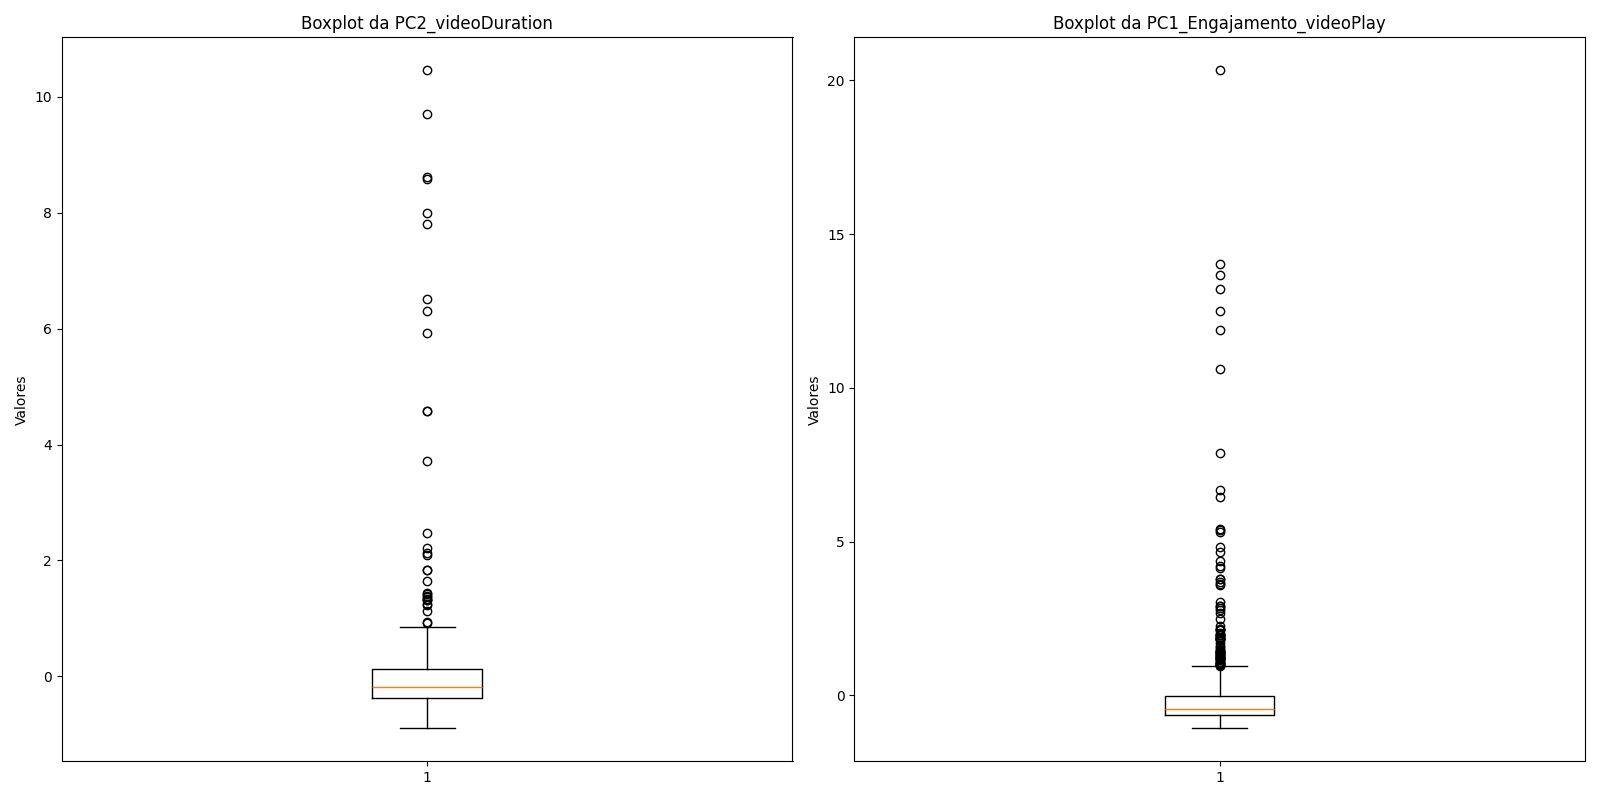
\includegraphics[width=1\textwidth]{Figuras/boxplot_do_dataframe.png}
    \caption{Boxplot dos Componentes Principais PC1 (Engajamento) e PC2 (Duração).}
    \label{fig:boxplot_pca}
\end{figure}

 O gráfico à direita, representando o PC1 (Engajamento\_videoPlay), revela que a grande maioria dos Reels possui um nível de engajamento concentrado em torno da mediana, que está próxima de zero. No entanto, a presença de uma longa cauda de outliers positivos, com valores que ultrapassam 20, é notável e característica de dados de engajamento, indicando que um número restrito de vídeos alcançou uma viralidade significativamente superior à média. De forma análoga, o gráfico à esquerda para o PC2 (videoDuration) mostra que a maioria dos vídeos tem uma duração padronizada e curta, também com uma cauda de outliers positivos que representam vídeos excepcionalmente mais longos. A existência proeminente de outliers em ambos os componentes sugere que tanto o engajamento viral quanto os vídeos de longa duração são eventos atípicos no conjunto de dados, o que justifica a utilização de algoritmos de clusterização robustos a outliers, como o DBSCAN, na etapa subsequente da análise.

\section{Clusterização}

Com base nos dois componentes principais, foi utilizada a ferramenta \texttt{AutoClusterHPO} para determinar o algoritmo de clusterização mais adequado. A ferramenta identificou o \textbf{DBSCAN} como o melhor algoritmo, com os parâmetros \texttt{eps=1.40} e \texttt{min\_samples=5}. O DBSCAN é um algoritmo baseado em densidade que é eficaz na identificação de clusters de formas arbitrárias e na detecção de outliers. A clusterização resultou em três grupos principais, como visualizado na Figura \ref{fig:clusters_pca}. A maioria dos Reels (792) foi agrupada no Cluster 0, enquanto 12 foram classificados como outliers (Cluster -1) e um pequeno grupo de 6 Reels formou o Cluster 1.

\begin{figure}[h!]
    \centering
    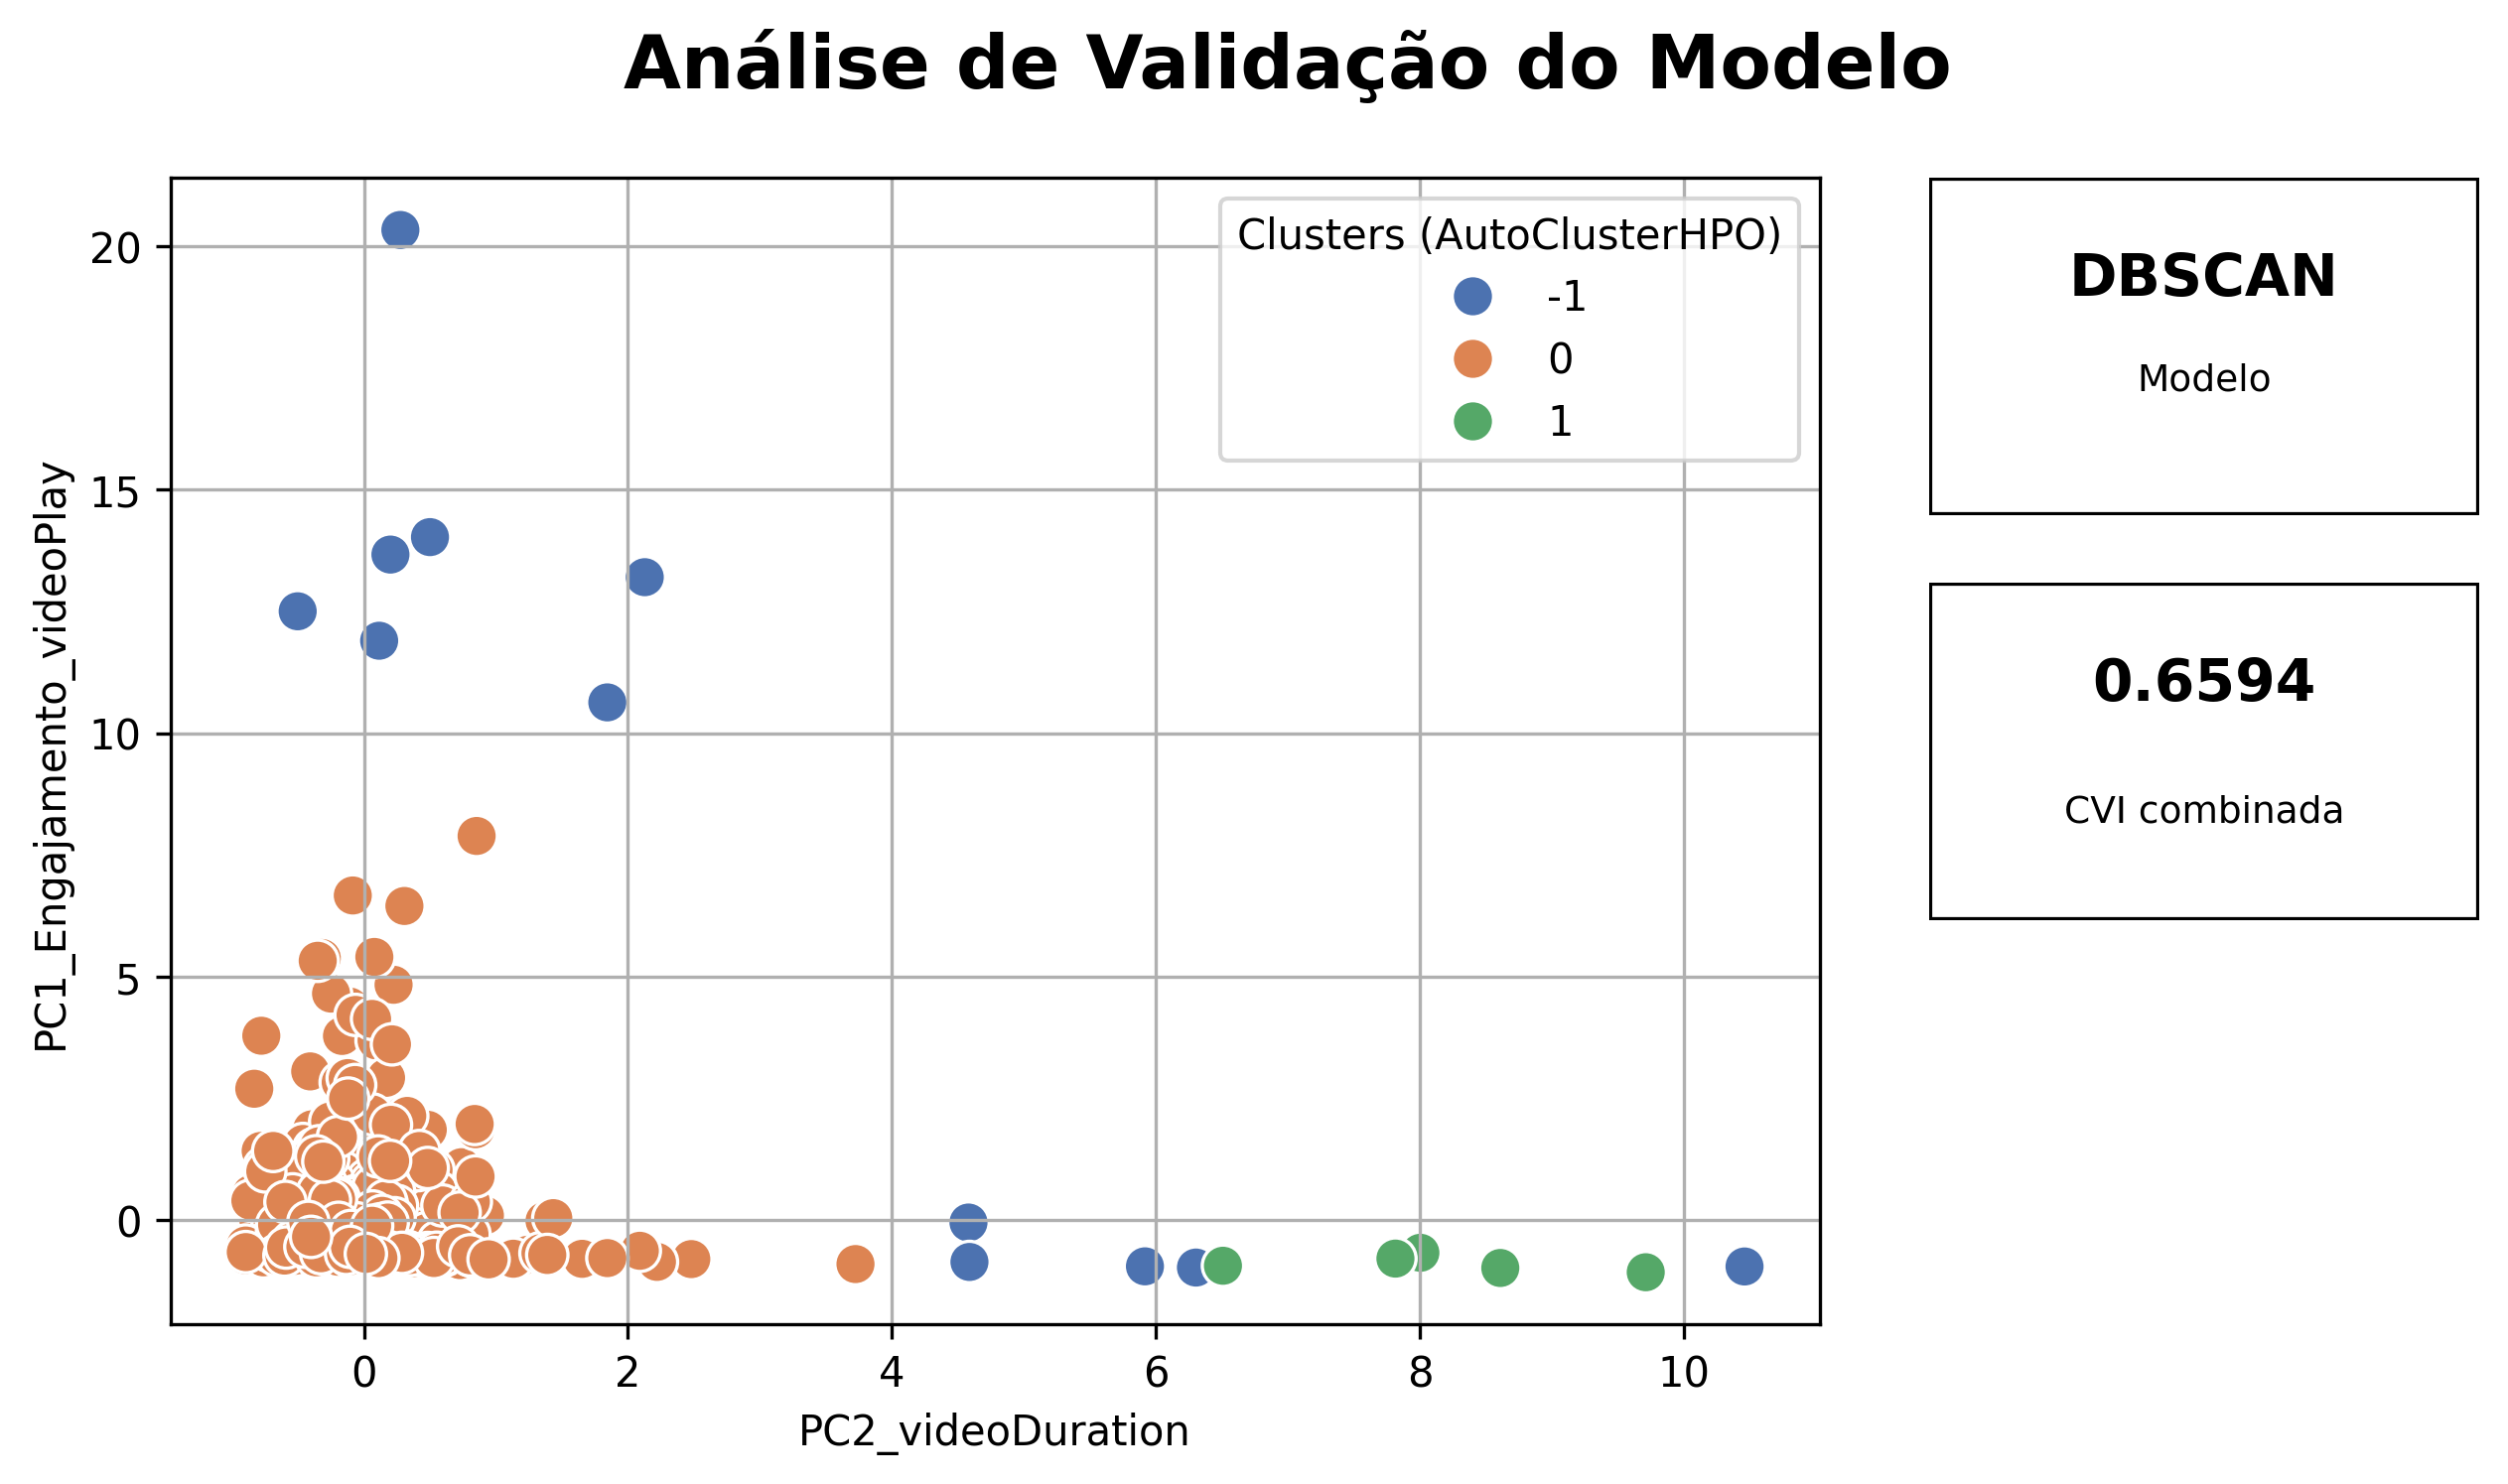
\includegraphics[width=1\textwidth]{Figuras/avaliacaoAutoCluster.png}
    \caption{Visualização dos Clusters com base nos Componentes Principais.}
    \label{fig:clusters_pca}
\end{figure}

A aplica\c{c}\~ao do framework \textit{AutoClusterHPO} para a an\'alise de dados dos Reels do Instagram, conforme visualizado na Figura 2, culminou na sele\c{c}\~ao autom\'atica do algoritmo DBSCAN como o modelo \'otimo, alcan\c{c}ando uma pontua\c{c}\~ao CVI combinada de 0.6594. A distribui\c{c}\~ao dos dados com base nos componentes principais revela uma segmenta\c{c}\~ao coesa, onde o modelo identificou dois clusters principais e um conjunto de outliers (r\'otulo -1). O cluster majorit\'ario (r\'otulo 0) agrupa os v\'ideos com menor dura\c{c}\~ao e engajamento, representando o comportamento padr\~ao na plataforma. De forma not\'avel, os pontos classificados como ru\'ido (-1) podem ser dividios em dois grupos, aqueles com valores elevados no componente principal associado ao engajamento (PC1) com baixa duração e aqueles com baixo engajamento e alta duração, indicando que o m\'etodo foi eficaz em isolar automaticamente os Reels de performance an\^omala.

O Cluster -1, embora contenha apenas 12 observações, contém os Reels de maior impacto. Uma de suas característica mais proeminente são a presença de vídeos com as métricas de engajamento elevadas, com uma média de 4.843 comentários e quase 90.000 curtidas, apesar de 25\% das publicações com menor engajamento apresentarem menos do que 103 comentários. O número de visualizações acompanha essa tendência, com uma média de 1,12 milhão. A duração dos vídeos neste cluster é bastante variada, com os vídeos variando desde 26 até 900 segundos. Mesmo com essa variação, foi possível analisar que os vídeos que contém mais do que 10 de PC1 apresentarem 83.44 segundos de média, variando de 26.32 até 180.03.

Representando a esmagadora maioria dos dados com 792 Reels, o Cluster 0 pode ser definido como o comportamento padrão da plataforma. Sua principal característica é a curta duração dos vídeos, com uma média de apenas 64,5 segundos. O engajamento é moderado e consistente com o que se esperaria de um conteúdo comum: uma média de 408 comentários, 5.543 curtidas e 117.883 visualizações. A baixa variabilidade na duração indica que este grupo é composto majoritariamente por vídeos curtos e rápidos.

O Cluster 1 é o menor grupo, com apenas 6 vídeos, e possui um perfil muito distinto. Sua característica definidora é a duração extremamente longa, com uma média de 721 segundos (aproximadamente 12 minutos). Em contrapartida, este cluster apresenta as piores métricas de desempenho. O engajamento é mínimo, com médias de 184 comentários e 1.554 curtidas, e o número de visualizações é o mais baixo de todos, com uma média de 29.323, sugerindo que vídeos muito longos no formato Reels não conseguem reter a atenção do público.

A principal diferença entre os clusters reside na aparente relação entre a duração do vídeo e o engajamento. O Cluster 0, de vídeos curtos, estabelece uma base de desempenho moderado, enquanto o Cluster 1 demonstra que estender excessivamente a duração leva a uma queda drástica no desempenho. Em contraste, o Cluster -1 mostra que o conteúdo de alto impacto pode performar excepcionalmente bem, com métricas de engajamento que são de 10 a 20 vezes maiores que as do Cluster 0.

Apesar das diferenças marcantes, uma semelhança notável pode ser encontrada na distribuição dos dados de engajamento dentro de cada cluster. Em todos os três grupos, a média de comentários e curtidas é consistentemente superior à mediana. Isso indica uma assimetria positiva em todos os segmentos, sugerindo que, mesmo dentro de um mesmo perfil de cluster, uma pequena parcela de vídeos tende a performar significativamente melhor que a maioria, criando uma "cauda longa" de popularidade.

\section{Análise de Sentimentos}

Para a classificação de sentimentos, foi utilizado um modelo pré-treinado robusto, o \texttt{cardiffnlp/twitter-xlm-roberta-base-sentiment}, através da biblioteca Transformers. Este modelo é especializado em textos de redes sociais e classifica cada comentário em uma de três categorias: \texttt{positive}, \texttt{neutral} ou \texttt{negative}. Além do rótulo, o modelo fornece um \textbf{score de confiança} (de 0 a 1), que indica o grau de certeza da classificação. 

A análise de sentimentos realizada neste projeto revelou uma predominância massiva de comentários positivos. As distribuições foram as seguintes:

\begin{figure}[h!]
    \centering
    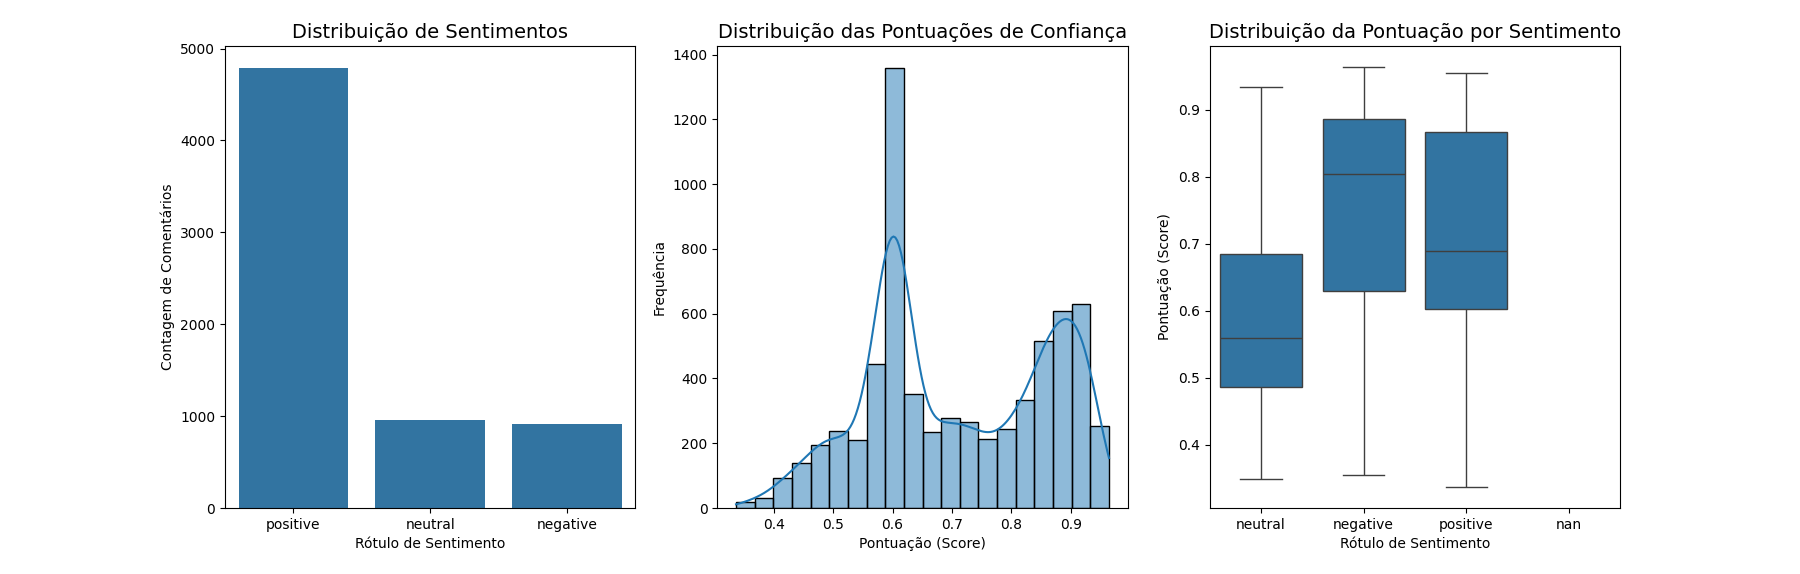
\includegraphics[width=\textwidth]{Figuras/sentiment_plots.png} 
    \caption{Visualizações da Análise de Sentimento: (a) Distribuição de Rótulos, (b) Distribuição dos Scores de Confiança, (c) Boxplot de Scores por Sentimento.}
    \label{fig:sentiment}
\end{figure}

Acima, é possível analisar que o Histograma de Scores de Confiança mostra que o modelo realizou a maioria de suas classificações com alta confiança (scores próximos de 1.0), indicando robustez. O Boxplot detalha essa confiança por categoria, mostrando que as classificações \texttt{positive} e \texttt{negative} possuem scores consistentemente mais altos do que a categoria \texttt{neutral}, o que é esperado, já que a neutralidade é semanticamente mais ambígua.

\subsection{Análise de Sentimentos por Perfis}

Após estabelecer o perfil de sentimento agregado do dataset e analisar a recepção qualitativa dentro dos clusters de performance, esta subseção avança a análise para o nível individual de cada perfil. O objetivo é dissecar a distribuição dos dados e identificar os outliers de performance qualitativa, movendo-se da análise de clusters para a de casos específicos. Ao isolar e examinar os cinco governadores com os maiores percentuais de comentários positivos e, em contrapartida, os cinco com os maiores percentuais de comentários negativos, esta análise busca validar empiricamente a tese central da Análise Exploratória de Dados (AED): a de que o desempenho digital é marcado por uma heterogeneidade extrema. Esta abordagem permite identificar quais figuras públicas específicas estão nas pontas da distribuição, ilustrando os perfis de comunicação que geram maior aprovação ou maior atrito público.

\begin{figure}[h!]
    \centering
    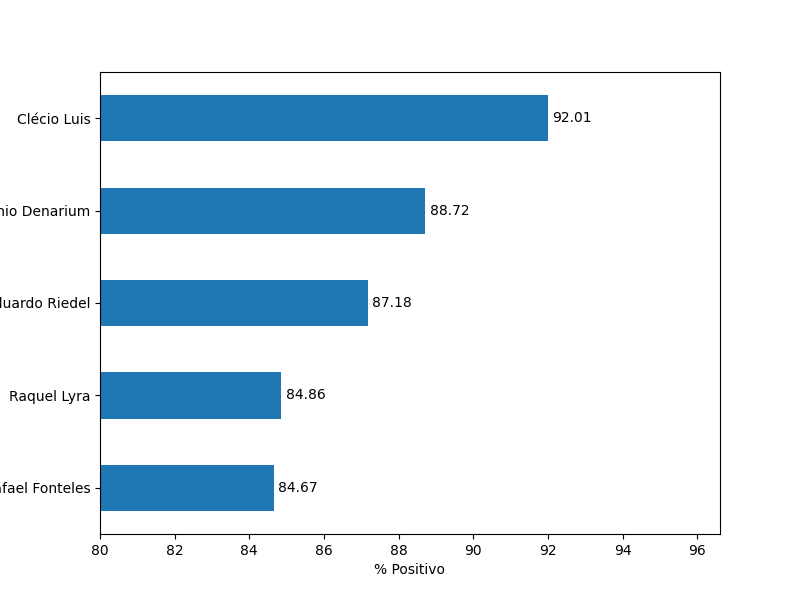
\includegraphics[width=0.5\textwidth]{Figuras/top_5_governadores_positivo.png} 
    \caption{Visualizações da Análise de Sentimento: 5 governadores com Maior percentual de comentários Positivos}
    \label{fig:sentiment}
\end{figure}

A análise do gráfico de barras horizontais, que ilustra os cinco governadores com maior percentual de comentários positivos, revela um desempenho de recepção qualitativa notavelmente elevado para este grupo de elite. Clécio Luís lidera o ranking de forma destacada, com 92,01\% dos comentários em suas publicações classificados como positivos, estabelecendo uma vantagem de mais de 3,2 pontos percentuais sobre o segundo colocado, Antonio Denarium (88,72\%). O grupo dos cinco primeiros é completado por Eduardo Riedel (87,18\%), Raquel Lyra (84,86\%) e Rafael Fonteles (84,67\%). É notável que todos os governadores neste top 5 mantêm um índice de positividade acima de 84\%, um patamar extremamente alto. Este resultado dialoga diretamente com a Análise Exploratória de Dados (AED) apresentada anteriormente na TCC (seção 5.1.1). A AED já havia estabelecido a presença de heterogeneidade extrema e assimetria positiva em todas as métricas quantitativas, como número de seguidores , soma de comentários e taxa de engajamento. Este novo gráfico de sentimento comprova que a mesma variabilidade se aplica à recepção qualitativa: assim como a AED identificou outliers quantitativos que distorcem a média (perfis com desempenho muito acima do padrão), o desempenho de Clécio Luís (92,01\%) representa um outlier qualitativo, validando a conclusão do TCC de que o desempenho dos governadores no Instagram não é uniforme, mas sim caracterizado por picos de performance excepcionais que se distanciam significativamente da mediana.

\begin{figure}[h!]
    \centering
    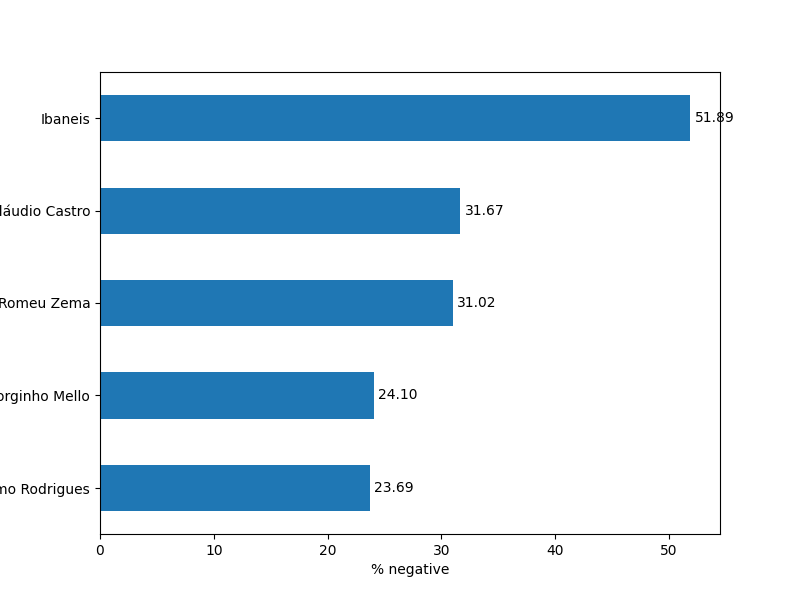
\includegraphics[width=0.5\textwidth]{Figuras/top_5_governadores_negativo.png} 
    \caption{Visualizações da Análise de Sentimento: Visualizações da Análise de Sentimento: 5 governadores com Maior percentual de comentários Negativos}
    \label{fig:sentiment}
\end{figure}

Em contrapartida, a análise dos cinco governadores com maior percentual de comentários negativos expõe o outro extremo da recepção pública. O governador Ibaneis apresenta-se como um outlier negativo proeminente, com 51,89\% de seus comentários classificados como negativos, indicando que mais da metade das interações em seu perfil são críticas. Este resultado é drasticamente superior aos demais, com Cláudio Castro (31,67\%) e Romeu Zema (31,02\%) formando um segundo patamar, seguidos por Jorginho Mello (24,10\%) e Tino Rodrigues (23,69\%). A existência de um perfil cuja recepção negativa supera os 50\% é uma ilustração clara da heterogeneidade extrema e da distribuição assimétrica que a Análise Exploratória de Dados (AED) do TCC (seção 5.1.1) já havia identificado. Assim como a AED revelou outliers de performance quantitativa (perfis com engajamento muito acima da média), este gráfico valida que também existem outliers qualitativos, onde a recepção do público é significativamente mais hostil do que a do restante do grupo, reforçando a conclusão de que o desempenho digital dos governadores é marcado por extremos em ambas as pontas.

A análise dos extremos da recepção qualitativa oferece uma conclusão contundente: a performance de sentimento dos governadores é tão ou mais assimétrica do que suas métricas de engajamento. A existência de um perfil como o de Clécio Luís, que alcança uma aprovação quase universal (92,01\% positiva), em conjunto com um perfil como o de Ibaneis, onde a hostilidade é majoritária (51,89\% negativa), invalida a noção de um "desempenho médio". Estes resultados reforçam de maneira inequívoca os achados da AED, demonstrando que o cenário digital não é um ambiente homogêneo, mas sim um conjunto de "microclimas" de recepção altamente polarizados. Fica evidente que o sucesso ou o fracasso na comunicação digital não se mede apenas pela quantidade de interações, mas pela qualidade drasticamente distinta dessa recepção, que varia de aprovação esmagadora a uma rejeição majoritária.

\subsection{Análise de Sentimentos por Clusters}

Para aprofundar a compreensão dos padrões de desempenho identificados, esta seção avança da segmentação métrica para a qualificação emocional, integrando os resultados da clusterização (seção 5.3) com os da análise de sentimentos (seção 5.4). Não basta identificar os clusters "Padrão" (Cluster 0), "Viral" (Cluster -1) e "Longo/Baixa Performance" (Cluster 1); é crucial dissecar a natureza da recepção do público dentro de cada um desses grupos. O objetivo desta análise cruzada é, portanto, mapear a distribuição percentual de comentários positivos, neutros e negativos para cada cluster. Esta abordagem sinérgica permite validar as características de cada grupo, revelando se a performance viral está associada à aclamação ou à controvérsia, e se a baixa performance está ligada à indiferença ou à rejeição

\begin{figure}[h!]
    \centering
    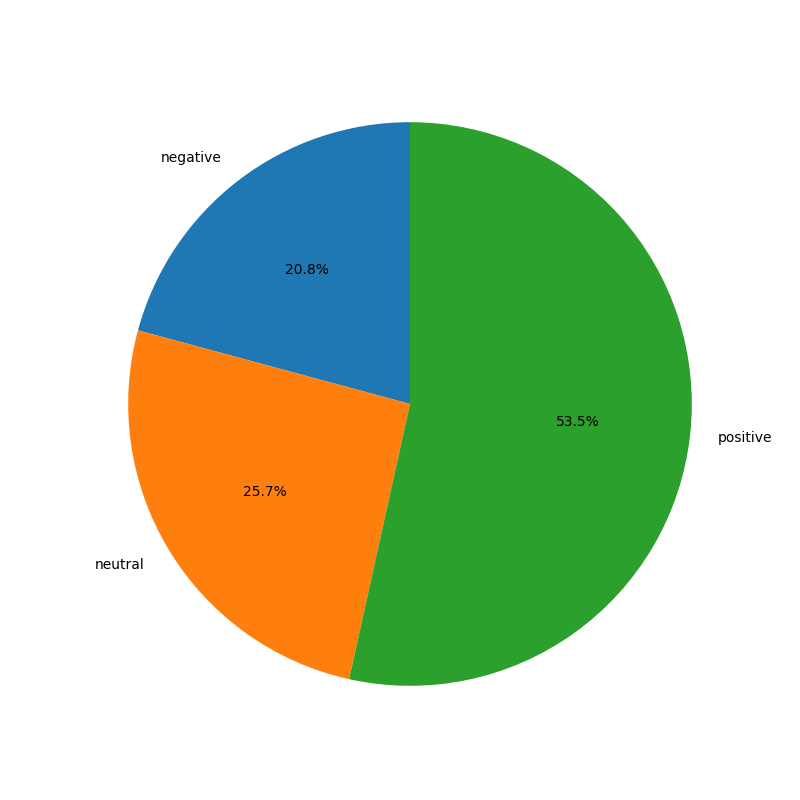
\includegraphics[width=0.4\textwidth]{Figuras/grafico_sentimentos_cluster-1.png} 
    \caption{Visualizações da Análise de Sentimento: Distribuição de Rótulos (Cluster -1)}
    \label{fig:sentiment}
\end{figure}

A análise de sentimentos para o Cluster -1, que o TCC identificou como o grupo de 12 Reels "outliers" de alto impacto e viralidade, revela uma dinâmica de recepção muito mais polarizada em comparação ao Cluster 0. Embora os comentários positivos ainda sejam majoritários (53,5\%), essa proporção é substancialmente menor (em comparação aos 72,3\% do Cluster 0). O insight mais relevante é o crescimento expressivo das reações não-positivas: os comentários negativos (20,8\%) e neutros (25,7\%) somam 46,5\% do total. Isso sugere que o conteúdo viral, caracterizado por um "Índice de Engajamento" (PC1) anômalo, não gera apenas aprovação, mas também atrai um volume significativamente maior de debate, críticas e reações ambíguas, refletindo a natureza muitas vezes controversa ou divisiva que impulsiona a própria viralidade.


\begin{figure}[h!]
    \centering
    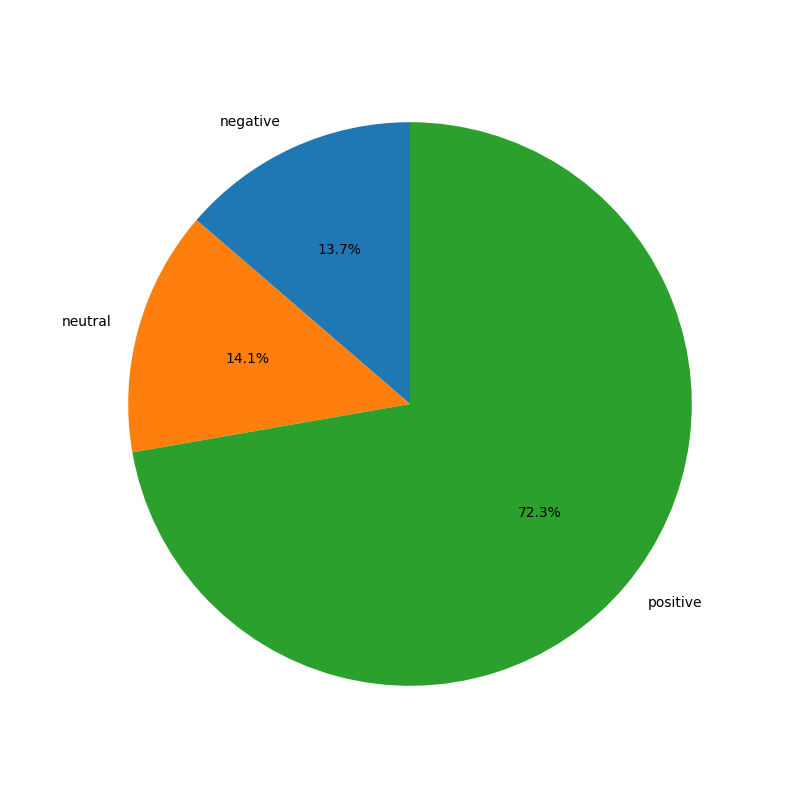
\includegraphics[width=0.4\textwidth]{Figuras/grafico_sentimentos_cluster0.png} 
    \caption{Visualizações da Análise de Sentimento: Distribuição de Rótulos (Cluster 0)}
    \label{fig:sentiment}
\end{figure}

A análise de sentimentos detalhada para o Cluster 0, o grupo mais representativo com 792 Reels, revela que o conteúdo "padrão" da plataforma é recebido de forma esmagadoramente positiva. Conforme o gráfico de pizza, 72,3\% dos comentários associados a este cluster foram classificados como positivos, indicando uma forte aprovação. Os sentimentos neutros (14,1\%) e negativos (13,7\%) são minoritários e apresentam proporções quase idênticas. Este resultado complementa e enriquece a definição anterior do Cluster 0: que os vídeos definidos pelo seu desempenho métrico "padrão" (curta duração, com média de 64,5 segundos, e engajamento moderado)  geram, de forma consistente, uma resposta emocional majoritariamente favorável do público.

\begin{figure}[h!]
    \centering
    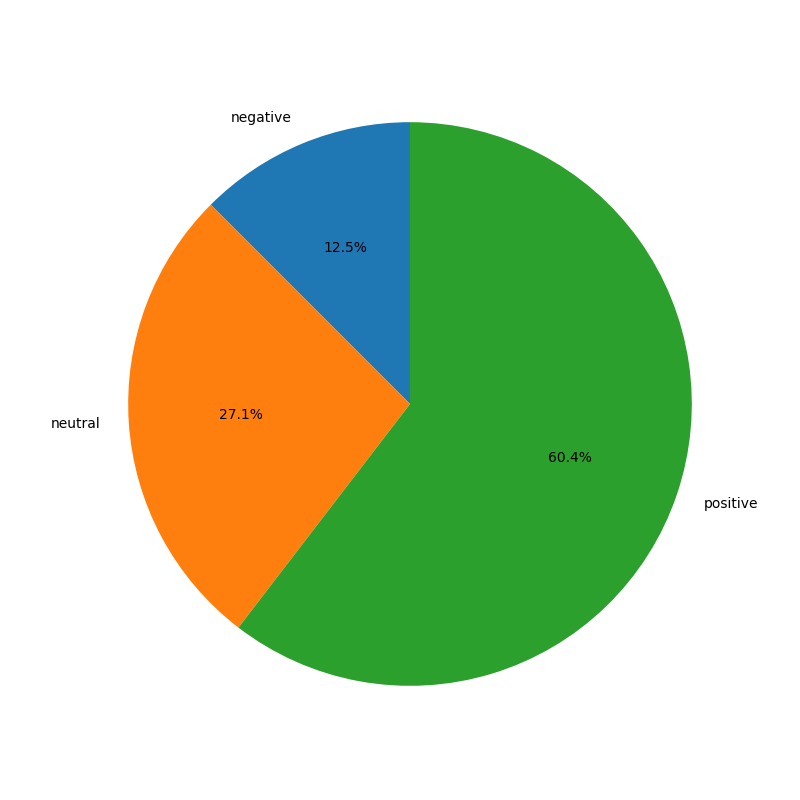
\includegraphics[width=0.4\textwidth]{Figuras/grafico_sentimentos_cluster1.png} 
    \caption{Visualizações da Análise de Sentimento: Distribuição de Rótulos (Cluster 1)}
    \label{fig:sentiment}
\end{figure}

A análise de sentimentos para o Cluster 1, o grupo de 6 Reels definido por sua duração extrema (média de 721 segundos) e desempenho de engajamento muito baixo, apresenta um perfil de recepção peculiar. Embora os comentários positivos ainda sejam a maioria (60,4\%), o dado mais distintivo é a alta proporção de comentários neutros (27,1\%), a maior entre todos os clusters. Combinado com o menor índice de comentários negativos (12,5\%), isso sugere um padrão claro: esses vídeos longos, que o TCC já havia identificado como de baixa performance, parecem falhar em gerar reações fortes. Eles não geram o alto engajamento do Cluster -1, mas também não atraem a negatividade; em vez disso, a audiência que interage é ou levemente positiva ou, mais significativamente, neutra, o que reforça a conclusão de que o conteúdo não consegue reter a atenção ou provocar um debate engajado, alinhando-se perfeitamente com suas métricas de desempenho fracas.

Com isso, conclui-se que a integração da análise de sentimentos com a clusterização é fundamental para desmistificar o real significado da performance métrica. Os resultados demonstram que "alto engajamento" não é sinônimo de "alta aprovação". O Cluster 0 (Padrão) estabelece a linha de base com uma recepção esmagadoramente positiva (72,3\%). Em nítido contraste, o Cluster -1 (Viral), dono das métricas mais fortes, revela-se o mais polarizado, com uma maioria positiva reduzida (53,5\%) e as maiores taxas de comentários negativos (20,8\%) e neutros (25,7\%), indicando que a viralidade foi impulsionada tanto pela aclamação quanto pela controvérsia. Por fim, o Cluster 1 (Longo/Baixa Performance) confirma sua ineficácia  ao apresentar a maior taxa de indiferença (27,1\% de comentários neutros), falhando em gerar reações emocionais fortes. A análise híbrida, portanto, qualifica os clusters, provando que o conteúdo padrão é aprovado, o viral é debatido, e o longo é ignorado.

\section{Modelagem de Tópicos com BERTopic}

A modelagem de tópicos identificou 50 temas distintos no corpus. As visualizações interativas fornecem insights profundos sobre a estrutura desses temas. O mapa da Figura 4 (Intertopic Distance Map) abaixo posiciona os tópicos em um espaço 2D com base em sua similaridade semântica. Cada círculo representa um tópico, e seu tamanho é proporcional à sua frequência.

\begin{figure}[h!]
    \centering
    % Substitua 'intertopic_map.png' pelo nome do arquivo de imagem salvo do seu notebook.
    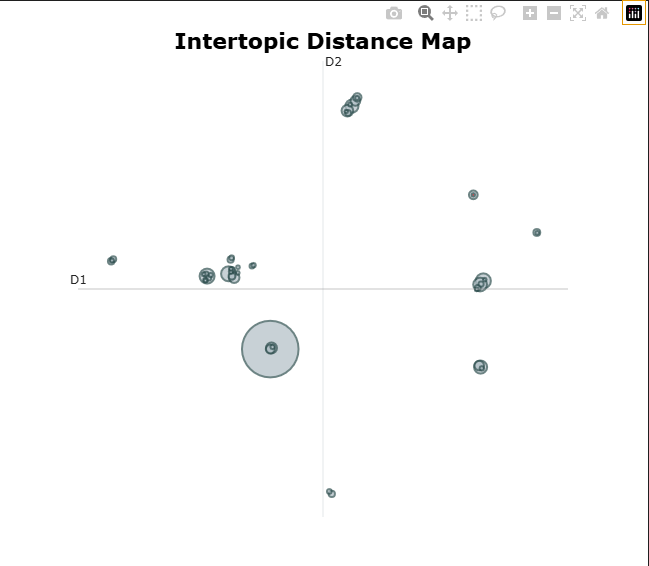
\includegraphics[width=0.9\textwidth]{Figuras/intertopic_map.png}
    \caption{Mapa de Distância Intertópica. Círculos próximos são semanticamente similares.}
    \label{fig:intertopic}
\end{figure}

A análise do mapa revela um \textbf{tópico dominante} (círculo grande), que representa a maioria dos comentários e é composto principalmente por expressões de apoio e emojis positivos (ex: aplausos, corações). Os demais tópicos, menores e mais dispersos, formam clusters que abordam assuntos mais específicos, como política, críticas a serviços públicos e pedidos de justiça.

Já o dendrograma de clusterização hierárquica (Figura 5) e o mapa de calor de similaridade (Figura 6) complementam a análise, mostrando como os tópicos se relacionam e podem ser agregados em meta-tópicos. Por exemplo, tópicos relacionados a críticas sobre concursos públicos e serviços de saúde, embora distintos, mostram-se semanticamente próximos e poderiam ser agrupados sob um tema maior de "Reivindicações de Serviços Públicos".

\begin{figure}[h!]
    \centering
    % Substitua 'hierarchy.png' pelo nome do arquivo de imagem salvo do seu notebook.
    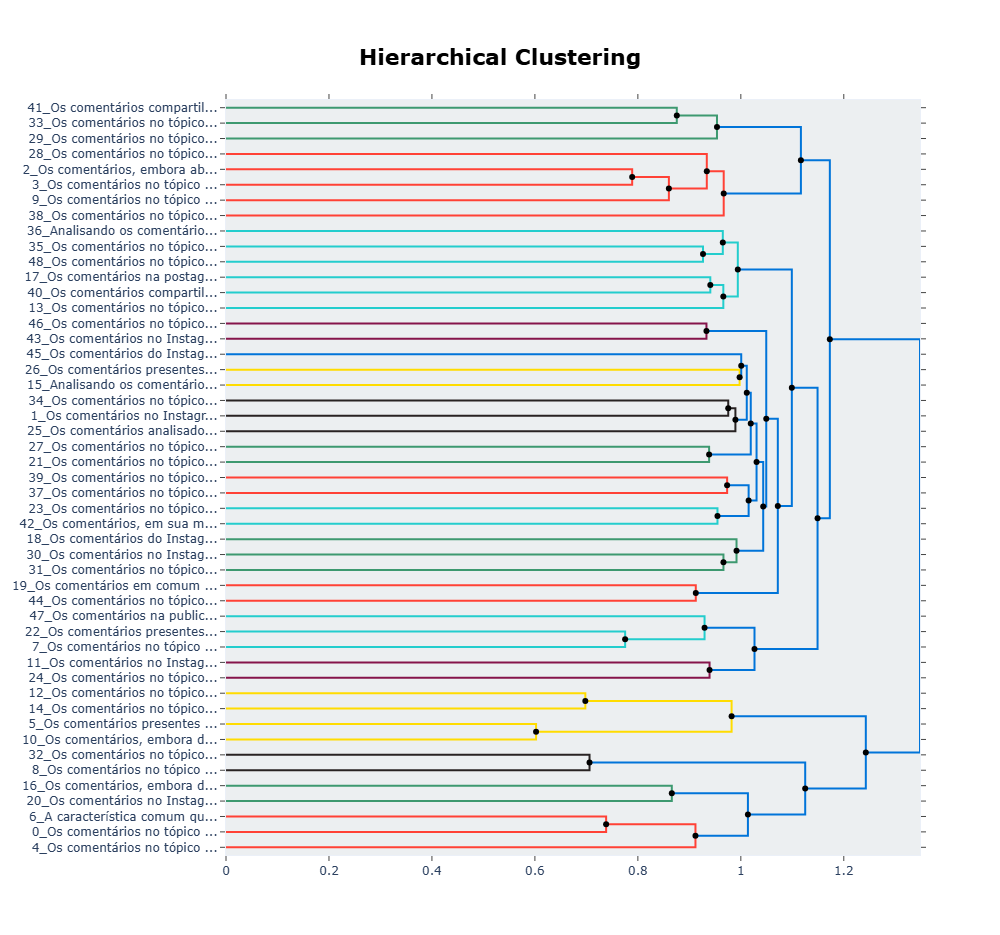
\includegraphics[width=\textwidth]{Figuras/hierarchy.png}
    \caption{Dendrograma da Clusterização Hierárquica dos Tópicos.}
    \label{fig:hierarchy}
\end{figure}

Com base na análise do dendrograma de clusterização hierárquica, a modelagem de tópicos mais coesa e distinta agruparia os comentários em quatro clusters principais. A justificativa para essa escolha reside em observar as distâncias horizontais em que os agrupamentos são formados. Ao traçar uma linha de corte vertical imaginária no eixo de distância em aproximadamente 1.1, identificamos quatro agrupamentos distintos que são fundidos em etapas posteriores com uma distância (dissimilaridade) significativamente maior, indicado pelas longas linhas horizontais que os conectam. O primeiro tópico hierárquico (topo, em tons de verde e vermelho) representa um tópico coeso. O segundo (meio-superior, em ciano, amarelo e preto) é o maior e mais diverso grupo, mas ainda assim claramente distinto dos demais. O terceiro (meio-inferior, em marrom e roxo) e o quarto (base do gráfico, em amarelo, cinza e vermelho) formam os dois últimos tópicos. Esta divisão em quatro grupos otimiza a modelagem, pois maximiza a similaridade dos comentários dentro de cada grupo, ao mesmo tempo que garante que os tópicos sejam significativamente diferentes entre si.

Os itens do primeiro tópico hierárquico (tópicos: 2, 3, 9, 29, 33, 36, 38, 41), têm em comum a descrição de comentários que expressam um forte sentimento de apoio, concordância e aprovação. A análise foca em reações positivas, como elogios a iniciativas e concordância com o conteúdo postado. Além disso, muitos itens descrevem ações que os usuários desejam realizar ou estão com dificuldade para fazer, como encontrar um link para inscrição ou cadastro, o que os une pelo tema de "ação do usuário". Quanto aos itens do segundo tópico hierárquico (tópicos: 1, 17, 21, 23, 25, 26, 28, 34, 35, 37, 39, 40, 42, 43, 45, 46), a principal característica deste grupo é a contextualização. As análises aqui presentes se concentram em identificar a origem dos comentários (plataforma, tipo de postagem) e frequentemente mencionam figuras de autoridade, como governadores, políticos ou outras personalidades públicas. O tema central é descrever a quem os comentários se dirigem e de onde vêm. Já os itens do terceiro tópico hierárquico (tópicos: 7, 11, 12, 14, 18, 19, 22, 24, 30, 31, 44, 47) agrupa as análises que se aprofundam nas qualidades e sentimentos dos comentários. Os textos descrevem o tom (irônico, crítico, de apoio), o estilo da linguagem, e as emoções predominantes, como admiração, insatisfação ou preocupação. O elo comum é a qualificação do discurso, indo além do tema para capturar a nuance e a subjetividade das mensagens. Por fim, os itens do quarto tópico hierárquico (tópicos: 4, 5, 6, 8, 10, 16, 20, 27, 32) são unidos por um forte viés de crítica, insatisfação e debate. As análises descrevem comentários que abordam problemas sociais, fazem reclamações, apontam divergências e expressam descontentamento com temas como gestão pública, segurança, educação e corrupção. É o cluster que representa a análise do discurso de oposição e conflito.

Abaixo pode-se analisar a matriz de similaridade entre os tópicos, que de forma semelhante ao dendograma, permitirá ao projeto agrupar tópicos semelhantes entre si. 

\begin{figure}[h!]
    \centering
    % Substitua 'heatmap.png' pelo nome do arquivo de imagem salvo do seu notebook.
    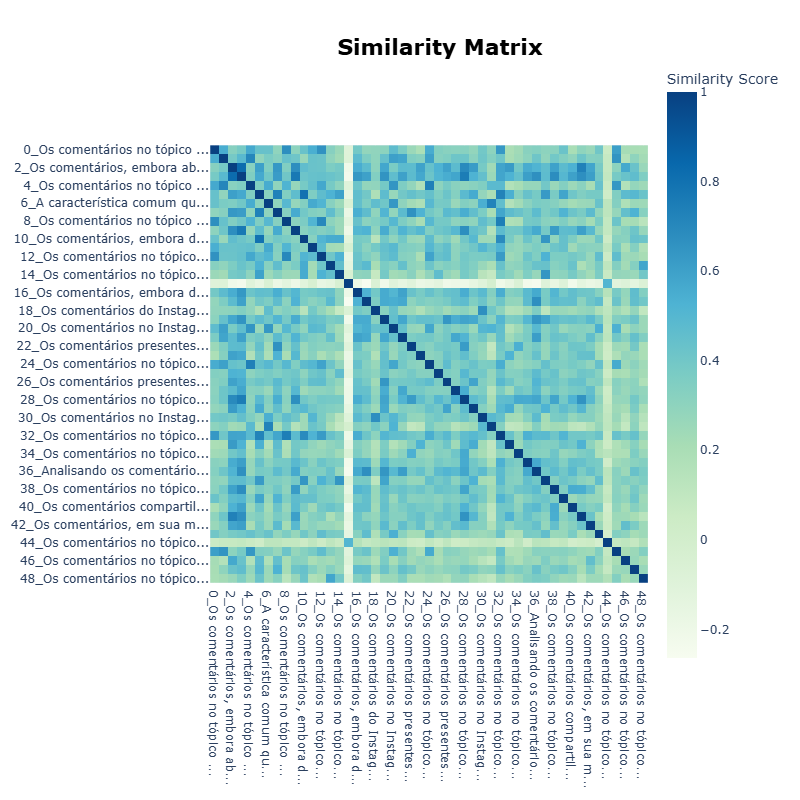
\includegraphics[width=\textwidth]{Figuras/heatmap.png}
    \caption{Matriz de Similaridade (Heatmap) entre os Tópicos.}
    \label{fig:heatmap}
\end{figure}

Analisando a matriz de similaridade, a modelagem de tópicos agruparia os comentários em aproximadamente quatro clusters principais, que são visualmente identificáveis como "quadrados" de cores mais escuras (tons de azul) ao longo da diagonal. A lógica para essa divisão é que os itens dentro de cada um desses quadrados demonstram uma alta pontuação de similaridade mútua, indicando que compartilham o mesmo tema central. O primeiro agrupamento pode ser visto no canto superior esquerdo (itens 0 a 8). Um segundo grupo coeso é observável no meio da matriz (aproximadamente itens 20 a 26). Um terceiro cluster é notado logo abaixo (itens 30 a 36). Finalmente, o agrupamento mais forte e coeso parece ser o do canto inferior direito (itens 40 a 48), que exibe os tons de azul mais escuros e consistentes, sugerindo uma altíssima similaridade interna. As áreas de cores mais claras (verdes/amarelas) entre esses blocos azuis representam a baixa similaridade entre os diferentes tópicos, justificando a sua separação em grupos distintos.

A aplicação do pipeline híbrido de NLP revelou com sucesso as principais características do corpus de comentários do Instagram. A análise de sentimentos indicou uma recepção majoritariamente positiva ao conteúdo dos Reels, com alta confiança do modelo classificador.

A modelagem de tópicos híbrida, combinando BERTopic e Gemini, provou ser excepcionalmente eficaz. Ela não apenas identificou a estrutura temática dos dados—com um tópico principal de reações positivas e diversos subtópicos específicos—mas também forneceu descrições contextuais e de fácil interpretação para cada tema. Esta abordagem representa um avanço significativo em relação aos métodos tradicionais, permitindo uma análise qualitativa mais profunda e a extração de insights acionáveis com maior facilidade. Os resultados demonstram o potencial da integração de modelos de embedding e modelos generativos para análises de texto complexas.



% !TEX root = ../TCC - CD e IA.tex
\chapter{Resultados}\label{Resultados}

% ==========================================================================
% ROTEIRO GERAL DO CAPÍTULO 6
% Propósito: este é o capítulo ACIONÁVEL. O cap. 5 apresentou a modelagem
% (o "motor"); aqui os resultados são organizados no funil COBRA-RACE e
% traduzidos em recomendações de growth. Fio condutor: sair da descrição
% ("o que os dados mostram") para a decisão ("o que a assessoria deve fazer").
% Não repetir a modelagem do cap. 5 — REFERENCIAR (\ref{}) e interpretar.
% ==========================================================================

% ROTEIRO (parágrafo de abertura do capítulo):
% - 1 parágrafo curto. Retomar a pergunta de pesquisa (do cap. 1) e anunciar
%   que este capítulo a responde aplicando o framework COBRA-RACE aos
%   resultados já obtidos no cap. 5.
% - Anunciar a estrutura do capítulo em 1 frase (as seções abaixo).

\section{Do Diagnóstico à Ação: Operacionalização do Funil de Engajamento}

% ROTEIRO:
% - Apresentar o framework COBRA-RACE já "montado" com OS SEUS dados.
% - Inserir uma TABELA (montar) que cruza: Estágio RACE | Nível COBRA |
%   métrica dos seus dados | cluster/figura correspondente.
%   Linhas: Reach->views(PC1); Act/Consumir->curtidas/cluster Padrão;
%   Convert/Contribuir->comentários+sentimento positivo;
%   Engage/Criar->comentários em debate (cluster Viral \ref{fig:sentiment-cluster-m1}).
% - Explicar que cada seção seguinte percorre um nível do funil.
% - Citar \cite{FEROZ2024} e \cite{MUNTINGA2011} ao apresentar a tabela.

\section{Segmentação de Publicações por Desempenho (Clusterização)}

% ROTEIRO:
% - Interpretar, à luz do growth, os 3 clusters de reels já obtidos (\ref{fig:clusters_pca}).
% - Retomar os números do cap.5/README: Cluster 0 "Padrão" (792 reels);
%   Cluster -1 "Viral" (12 reels, ~4.843 comentários, ~90k curtidas, 1,12M views);
%   Cluster 1 "Longo" (6 reels, ~721s de duração média).
% - NÃO reexplicar PCA/DBSCAN (está no cap.5) — referenciar \ref{tab:pca_loadings}.
% - Fechar cada cluster com sua LEITURA de growth (Padrão=aprovado,
%   Viral=debatido/polarizado, Longo=ignorado/indiferença).

\subsection{Clusterização de Publicações do Feed}

% ROTEIRO (PENDENTE DE EXECUÇÃO — você disse que vai gerar):
% - Rodar AutoClusterHPO também sobre os posts do FEED (hoje só há de reels).
% - Preencher com: nº de clusters encontrados, algoritmo eleito, score CVI,
%   perfil de cada cluster. Inserir figura análoga à \ref{fig:clusters_pca}.
% - Comparar com os clusters de reels: os padrões se repetem no feed?

\subsection{Clusterização de Perfis dos Governadores}

% ROTEIRO (PENDENTE DE EXECUÇÃO — você disse que vai gerar):
% - Rodar clusterização sobre as MÉTRICAS AGREGADAS por perfil
%   (tabela governor_engagement / \ref{tab:matriz_correlacao}).
% - Preencher: quantos grupos de governadores emergem, o que caracteriza
%   cada grupo (ex: "alto alcance/baixa conversão"), quais governadores em cada.
% - Este é o nível de segmentação à la Flesch \cite{FLESCH2017}: nomear os
%   grupos em termos funcionais se possível (loyalist-heavy, critic-heavy...).

\section{Qualificação dos Segmentos pelo Sentimento}

% ROTEIRO:
% - Cruzar clusters x sentimento (a etapa que "prova a tese", README seção 2.5).
% - Inserir a TABELA de distribuição de sentimento por cluster (montar a partir
%   das figuras \ref{fig:sentiment-cluster-m1}, \ref{fig:sentiment-cluster-0},
%   \ref{fig:sentiment-cluster-1}):
%   Cluster 0: 72,3% pos / 14,1% neu / 13,7% neg
%   Cluster -1 (Viral): 53,5% pos / 25,7% neu / 20,8% neg  <- polarizado
%   Cluster 1 (Longo): 60,4% pos / 27,1% neu / 12,5% neg   <- indiferença
% - Interpretar: alto engajamento (Viral) NÃO é alta aprovação. Este é o
%   achado central — conectá-lo explicitamente à crítica das vanity metrics
%   \cite{FEROZ2024} feita no referencial (seção 3.2).

\section{Discurso da Assessoria versus Reação do Público (Tópicos)}

% ROTEIRO:
% - Este é o contraste NOVO e mais rico. Precisa dos tópicos das legendas/
%   transcrições (discurso oficial) vs. tópicos dos comentários (público).
% - Comentários: retomar os 50 tópicos do BERTopic (\ref{fig:intertopic},
%   \ref{fig:hierarchy}, \ref{fig:heatmap}) já obtidos.
% - Legendas/transcrições (PENDENTE — vêm da API): rodar BERTopic sobre elas.
% - Montar a análise de GAP: temas que a assessoria pauta mas o público
%   ignora; temas que o público levanta mas a assessoria não aborda.
% - Este gap é a matéria-prima das recomendações da seção seguinte.

\section{Métricas de Crescimento e Priorização}

\subsection{North Star Metric: Engajamento Positivo Qualificado}

% ROTEIRO:
% - Definir a fórmula da NSM (a detalhar em bloco próprio — ver conversa).
%   Ideia: (comentários positivos / comentários totais) ponderado por alcance.
% - Calcular a NSM por perfil a partir de governor_sentiment + governor_engagement.
% - Contrastar o ranking por NSM com o ranking por engajamento bruto —
%   mostrar que mudam de ordem (prova de que a métrica importa).
% - Ancorar em \cite{FEROZ2024} e no precedente de Loyalty Rate (a citar).

\subsection{Retenção e Crescimento da Audiência (CMGR)}

% ROTEIRO:
% - Usar governor_engagement_history (tabela append, já existe) para calcular
%   crescimento ao longo do tempo, à la Flesch \cite{FLESCH2017}.
% - Se houver poucos pontos temporais ainda, declarar honestamente a limitação
%   e apresentar o método pronto para quando houver mais coletas.

\subsection{Priorização de Temas (Score ICE)}

% ROTEIRO:
% - Rankear os 50 tópicos por um score simples: Impacto (alcance do tópico x
%   sentimento positivo) x Confiança x Facilidade.
% - Entregar uma tabela "top temas a produzir" — saída diretamente acionável.

\section{Estudo de Caso Aplicado: Recomendações por Perfil}

% ROTEIRO:
% - AQUI o framework "paga" tudo. Escolher 2-3 governadores dos EXTREMOS já
%   identificados no cap.5:
%   * Clécio Luís (92,01% positivo, \ref{fig:sentiment-top5-positivo})
%   * Ibaneis (51,89% negativo, \ref{fig:sentiment-top5-negativo})
%   * (opcional) um caso mediano de contraste.
% - Para CADA um, aplicar o funil completo: em que estágio a audiência trava?
%   Qual o gap discurso x reação? O que a NSM revela? E então:
%   3-5 recomendações CONCRETAS de growth ("produzir mais X", "abandonar
%   formato Y", "o tema Z converte e está subexplorado").
% - Este é o núcleo do valor prático do TCC. Ser específico e acionável.

\section{Validação: Abordagem Híbrida versus Análises Isoladas}

% ROTEIRO (responde ao objetivo específico nº 6):
% - Argumentar, com os resultados em mãos, o que CADA técnica isolada NÃO
%   veria e que a integração revelou:
%   * só sentimento: veria "Ibaneis tem muita crítica" mas não em qual formato/tema.
%   * só tópicos: veria os temas mas não a valência nem o desempenho.
%   * só clusterização: veria grupos de performance mas não o conteúdo/reação.
% - Fechar com o achado que só o cruzamento permite: "engajamento != aprovação".

% !TEX root = ../TCC - CD e IA.tex
\chapter{Conclusões}\label{Conclusões}

% ==========================================================================
% ROTEIRO GERAL DO CAPÍTULO 7
% Sintetizar sem repetir. Responder à pergunta de pesquisa do cap.1 de forma
% direta. Não introduzir resultado novo aqui — só consolidar.
% ==========================================================================

% ROTEIRO (parágrafo de abertura):
% - Retomar a pergunta de pesquisa e afirmar, em 1 parágrafo, como o trabalho
%   a respondeu: a metodologia híbrida, organizada em funil, virou ferramenta
%   de decisão para assessorias.

\section{Síntese das Contribuições}

% ROTEIRO:
% - Recuperar as duas frentes (metodológica e prática) do cap.1.
% - Metodológica: pipeline híbrido integrando 3 técnicas sobre 3 fontes
%   textuais e múltiplos níveis de agregação; refino de tópicos via LLM.
% - Prática: o framework COBRA-RACE, a NSM, o contraste discurso x reação,
%   e as recomendações por perfil.
% - Retomar o achado central: alto engajamento != alta aprovação.
% - Amarrar cada contribuição ao objetivo específico correspondente (1 a 8).

\section{Limitações do Estudo}

% ROTEIRO (ser honesto — a banca valoriza):
% - Dados observacionais, não experimentais (sem A/B): não se estabelece causalidade.
% - Recorte temporal da coleta / poucos pontos para série histórica de CMGR.
% - Transposição de construtos comerciais (COBRAs) ao político — ressalva já
%   feita no cap.3, retomar aqui.
% - Dependência de modelo de sentimento pré-treinado (possíveis vieses em PT-BR,
%   ironia/sarcasmo em comentários políticos).
% - Refino de tópicos via LLM introduz etapa não-determinística.

\section{Sugestões para Trabalhos Futuros}

% ROTEIRO:
% - Teste A/B de formato/tema fechando o loop de aprendizado de growth.
% - Modelo preditivo de engajamento (prever cluster Padrão/Viral/Longo antes de postar).
% - Extensão a outras figuras políticas / outras plataformas (comparabilidade).
% - Análise temporal de retenção com mais coletas.
% - Detecção de ironia/sarcasmo para refinar a análise de sentimento política.

\section{Considerações Finais}

% ROTEIRO:
% - 1 parágrafo de encerramento. Voltar ao "porquê" do trabalho: dar a
%   assessorias uma ferramenta que substitui a intuição por evidência, num
%   ambiente digital decisivo para a democracia. Fechar com a nota de que
%   correlação não implica causalidade — postura que o trabalho manteve.

% ----------------------------------------------------------
\pagebreak

% ----------------------------------------------------------
% Bibliografia
% ----------------------------------------------------------
\bibliography{IESB-CDeIA-Bibliografia}

% ----------------------------------------------------------
% Anexos
% ----------------------------------------------------------

% ----------------------------------------------------------
% Anexos
% ----------------------------------------------------------
% ---
% Inicia os anexos
% ---
\begin{anexosenv}
    % Imprime uma página indicando o início dos anexos
    \partanexos
    % ---
    \chapter{Dicionário de Dados}
    % ---
    A seguir estão descritos todos os bancos de dados, suas tabelas e variáveis
    % ---
    \chapter{Códigos dos Programas}
    % ---
    A seguir estão descritos todos os códigos de programas desenvolvidos
    % ---
    \chapter{Notebooks Python}
    % ---
    A seguir estão descritos todos os notesbooks Python utilizados para gerar as análises e resultados deste trabalho

\end{anexosenv}

% ----------------------------------------------------------
\end{document}